\chapter{Architectural Design}

\section{Overview}
The system will be developed from scratch and it will completely replace the legacy system. \newline

\vspace{0.8em}
\begin{figure}[H]
	\centering
	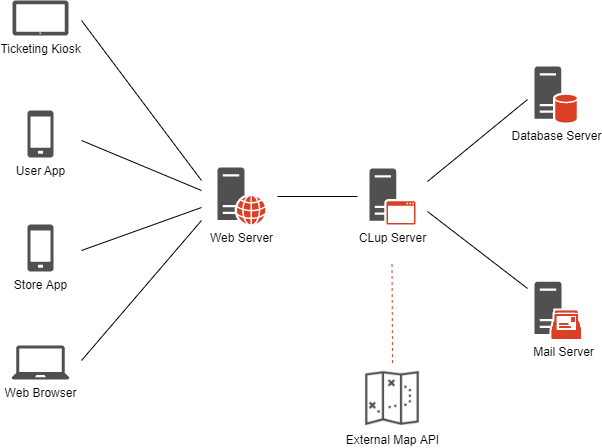
\includegraphics[scale=0.45]{overview_diagram}
	\caption{CLup system diagram.}
\end{figure}

It is composed by a client part and a server part:
\begin{itemize}
	\item \textbf{Server side:}
	\begin{itemize}
		\item \textit{Application Server (CLup Server):} server where all the logic is located. It communicates with other servers and is the central point of the system.
		\item \textit{Web Server:} server used for the communication with the clients.
		\item \textit{Database Server:} server where all data are stored.
		\item \textit{Mail Server:} server used to send confirmation emails about the bookings.
		\item \textit{External map API:} API used to retrieve data about the distance of the user from the store. This information will be used to inform the user of when leave the current place.
	\end{itemize}
	\item \textbf{Client side:}
	\begin{itemize}
		\item \textit{User App:} Application installed on customers smartphone. It allows to retrieve a ticket or book a visit.
		\item \textit{Store App:} Application installed on employees smartphone. It allows to validate store passes.
		\item \textit{Ticketing Kiosk:} Tablet installed at the entrance of the store to which a printer is attached. It has installed a modified version of the customer app which is able to print the ticket on place.
		\item \textit{Web Browser:} Used by store employees and managers to access the web dashboard.
	\end{itemize}
\end{itemize}

\section{Component view}

\subsection{High Level}
The following component diagram highlights all the components of the system and describes both his internal and external interactions.
A general overview of the whole system is shown in \clupautoref{fig:cmp_high_level}. Further details will be provided in the subsequent diagrams.

\begin{figure}[H]
	\centering
	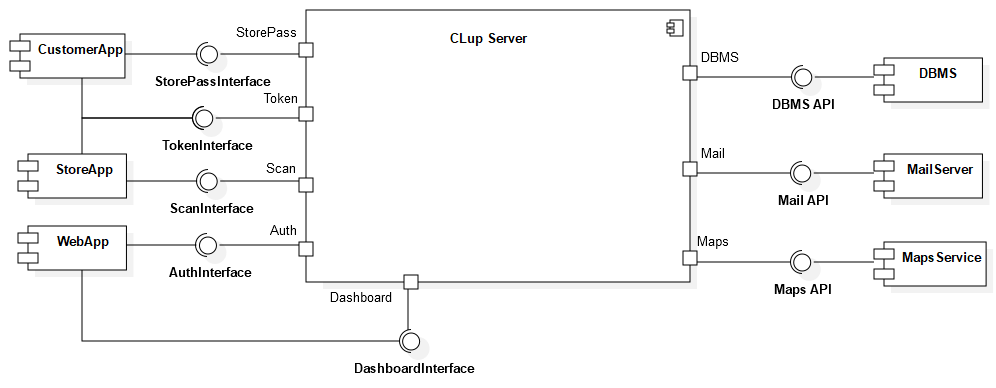
\includegraphics[origin=c,width=\textwidth]{component/cmp_high_level}
	\caption{\textit{High level} component diagram.}
	\label{fig:cmp_high_level}
\end{figure}

The components in \clupautoref{fig:cmp_high_level} are:
\begin{itemize}
	\item \textbf{CLup Server}: contains the business logic of the entire system. This component offers to both customers and supermarkets the features of \textit{CLup}. On the one side, the interfaces provided by this components allow the client side (mobile apps and web app) to communicate with the server. On the other side, it interfaces with external systems such as the database server, the email server and the maps service. Further detailed in \clupautoref{fig:cmp_clup_server}.
	
	\item \textbf{Customer App}: represents the mobile application installed on the customers' devices. Upon authentication via the \textbf{Token Interface}, it allows customers to access the store pass functions of \textit{CLup} by using the \textbf{StorePass Interface}.
	
	\item \textbf{Store App}: represents the mobile application	installed on the devices of the store. Upon authentication with credentials via the \textbf{Token Interface}, it allows the store employees to access the scan functions of \textit{CLup} by using the \textbf{Scan Interface}.
	
	\item \textbf{Web App}: represents the web application reachable by any modern web browser by the store managers. Upon authentication with credentials via the \textbf{Auth Interface}:
	\begin{itemize}
		\item allows the store managers to access the dashboard functions of \textit{CLup} by using the \textbf{Dashboard Interface};
		\item allows CLup admins to register and delete stores from the system by using the \textbf{Dashboard Interface}.
	\end{itemize}
	
	\item \textbf{Database Server}:	provides the interface to the \textit{CLup Server} to deal with the data management process. 
	
	\item \textbf{Mail Server}: provides the interface to the \textit{CLup Server} to deal with the email sending and receiving services needed. The email system is necessary for both the process of registration of stores and the validation of the customers' booking.
	
	\item \textbf{Maps Service}: provides the interface to the \textit{CLup Server} to deal with the maps data. It is required to retrieve the best possible path between two positions and to calculate the \textit{leave-at-time}.
\end{itemize}

\clearpage

\subsection{CLup Server}
The following component diagrams describe the internal structure of the application server, which contains the business logic of the system.

\begin{figure}[H]
	\centering
	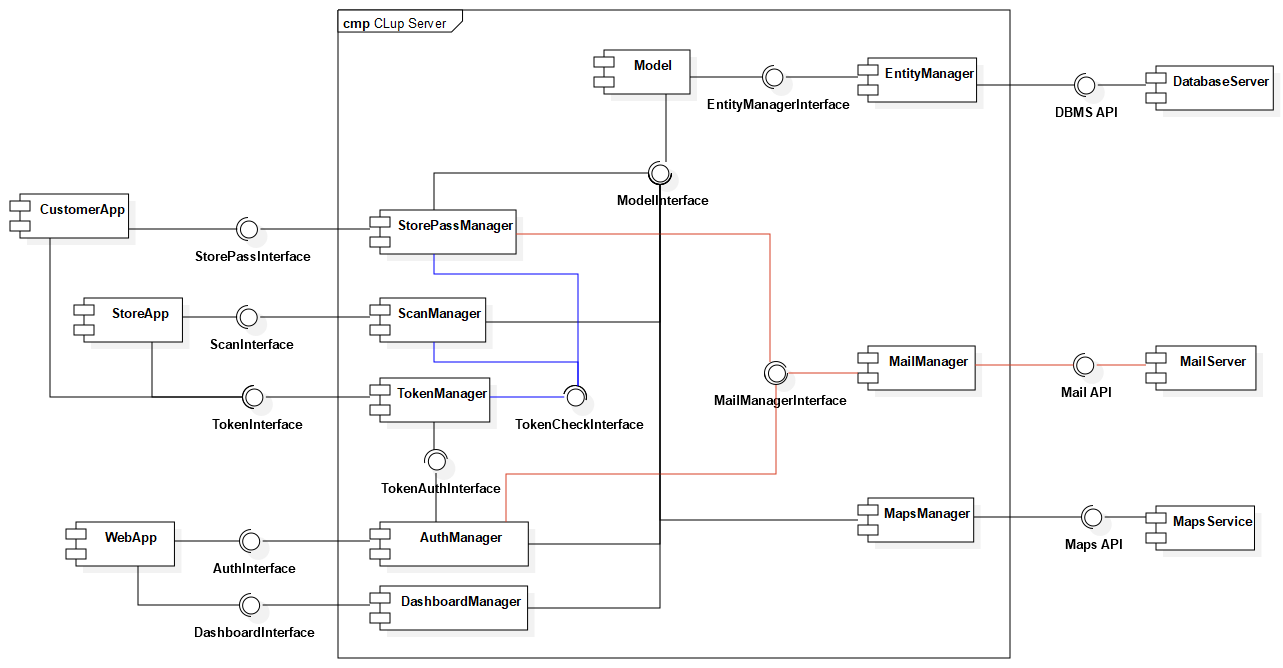
\includegraphics[angle=90,origin=c,height=\textwidth]{component/cmp_clup_server}
	\caption{\textit{CLup Server} component diagram.}
	\label{fig:cmp_clup_server}
\end{figure}
\clearpage

The components in \clupautoref{fig:cmp_clup_server} are:
\begin{itemize}
	\item \textbf{StorePassManager}: handles the main feature offered to the customers to line up at stores. In particular, it manages all the logic of store passes life-cycle, from their creation to expiration and deletion. Further detailed in \clupautoref{fig:cmp_store_pass}.
	
	\item \textbf{ScanManager}: handles the main feature offered to the store employees. In particular, it manages all the logic of store passes scan and validation. Further detailed in \clupautoref{fig:cmp_scan}.
	
	\item \textbf{TokenManager}: deals with token generation and validation for the mobile applications. It interfaces with the AuthManager through the \textbf{TokenAuth Interface} to integrate the authentication when using credentials.
	
	\item \textbf{AuthManager}: deals with the authentication of CLup admins, store managers and employees. Allows the generation of store credentials. Further detailed in \clupautoref{fig:cmp_auth}
	
	\item \textbf{DashboardManager}: handles the main feature offered to the store managers. In particular, it offers a dashboard that allows:
	\begin{itemize}
		\item \textbf{Store managers}:
				\begin{itemize}
					\item to monitor the status of their store;
					\item to change the maximum number of people inside the store;
					\item to manage the bookings of the customers.
				\end{itemize}
			
		\item \textbf{Store employees}: to view the next store passes that will be called.
		\item \textbf{CLup admins}: to manage the creation and deletion of stores.
	\end{itemize}
	
	\item \textbf{Model}: high-level component which represent the data on the server and acts as a mask to the database server. Since it is the entry point to the data, almost every component needs to interface with this one.
	
	\item \textbf{EntityManager}: deals with all the management of the data needed by the system. It perform object-relational mapping to the \textbf{Model} component and uses the methods provided by the \textbf{DBMS API} to execute queries on the database.
	
	\item \textbf{MailManager}: interfaces with the Mail API to send emails.	
	
	\item \textbf{MapsManager}: deals with the maps data. It retrieves the best possible path between two positions and to calculate the \textit{leave-at-time}.
\end{itemize}

\clearpage

\subsection{Store Pass Manager}

\begin{figure}[H]
	\centering
	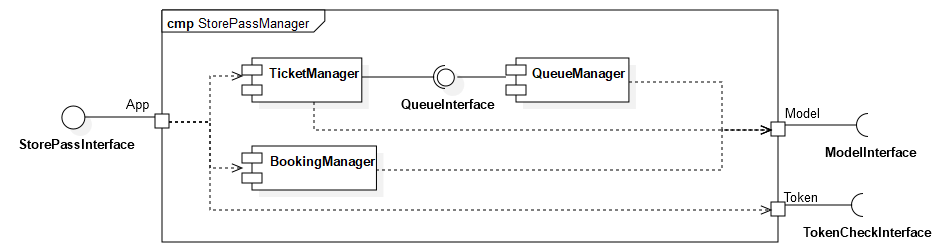
\includegraphics[origin=c,width=\textwidth]{component/cmp_store_pass}
	\caption{\textit{Store Pass Manager} component diagram.}
	\label{fig:cmp_store_pass}
\end{figure}

The components in \clupautoref{fig:cmp_store_pass} are:
\begin{itemize}
	\item \textbf{TicketManager}: handles the tickets creation for a specific store. Provides methods to the Customer App to update the current status of the queue and through the \textbf{Model Interface} can access the maps data to provide the leave-at-time.
	
	\item \textbf{BookingManager}: handles the booking creation for a specific store. Provides methods to the Customer App to update the current status of the queue and through the \textbf{Model Interface} can access the maps data to provide the leave-at-time.
	
	\item \textbf{QueueManager}: deals with the queue management for each stores subscribed and calculates the estimated waiting time in queue. It offers an interface to the \textit{Ticket Manager} which allows it to add and remove tickets from the queues. Furthermore, the \textbf{ViewStatusInterface} provides the current status of the queue.
\end{itemize}


\subsection{Auth Manager}

\begin{figure}[H]
	\centering
	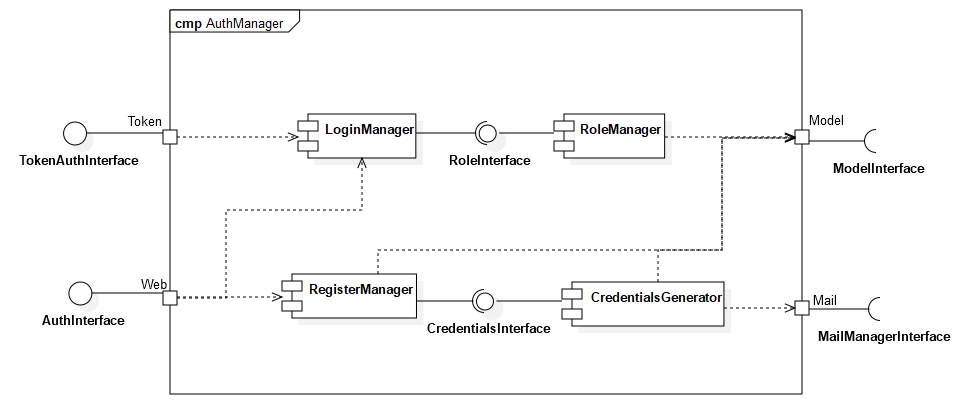
\includegraphics[origin=c,width=\textwidth]{component/cmp_auth}
	\caption{\textit{Auth Manager} component diagram.}
	\label{fig:cmp_auth}
\end{figure}

The components in \clupautoref{fig:cmp_auth} are:
\begin{itemize}
	\item \textbf{LoginManager}: handles the login and credentials check of CLup admins, store managers and store employees in the system. It interfaces with the RoleManager through the \textbf{RoleInterface} to give the right permissions to the logged user.
	
	\item \textbf{RegisterManager}: handles the registration of new stores in the system. It communicate with the Model in order to save the registered stores.
	
	\item \textbf{RoleManager}: handles the role based access control (RBAC): an authorization scheme that grants access rights based on the role of the use. In particular, this components grants user authentication and authorization:
	\begin{itemize}
		\item Authentication: request and verify the identity of CLup admin, store managers and employees attempting to login using a usercode and password;
		\item Authorization: verify the permissions of the logged user to perform any requested action (e.g. adding or removing a store, creating a new item category, etc.) before performing it.
	\end{itemize}
		
	\item \textbf{CredentialsGenerator}: handles the credentials generation when a CLup Admin adds a new store to the system. It interfaces with the MailManager to send the credentials to the store PEC address.
\end{itemize}


\subsection{Scan Manager}

\begin{figure}[H]
	\centering
	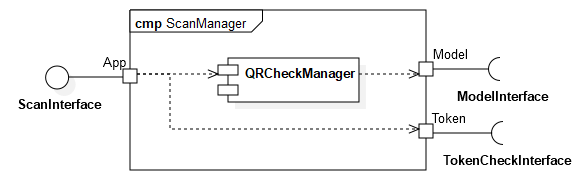
\includegraphics[origin=c,width=\textwidth]{component/cmp_scan}
	\caption{\textit{Scan Manager} component diagram.}
	\label{fig:cmp_scan}
\end{figure}

The components in \clupautoref{fig:cmp_scan} are:
\begin{itemize}
	\item \textbf{QRCheckManager}: it handles the scanning and validation process of QR codes. The scanned code validity will be checked versus the one stored in the Model via the ModelInterface.
\end{itemize}
\clearpage

\section{Deployment view}
The system presents a three tier architecture \clupautoref{fig:depl_diag}:
\begin{itemize}
	\item \textbf{Tier 1: presentation tier}. The Customer App is installed on compatible Android or iOS phones. Distribution of the appropriate executable will be handled by the corresponding app stores. For the Local Ticketing Kiosk, a custom non-public executable will be installed on an Android tablet.\newline
	The Store App is installed on Android or iOS phones and will not be publicly available.\newline
	Finally, the Web App will be accessible through web browser by connecting to a dedicated website.
	
	\item \textbf{Tier 2: logic tier}. The CLup Server App is installed on a dedicated server with a running instance of Apache TomEE 8.
	
	\item \textbf{Tier 3: data tier}. All data is stored in a persistent way into a MySQL database.
\end{itemize}


\begin{figure}[H]
	\centering
	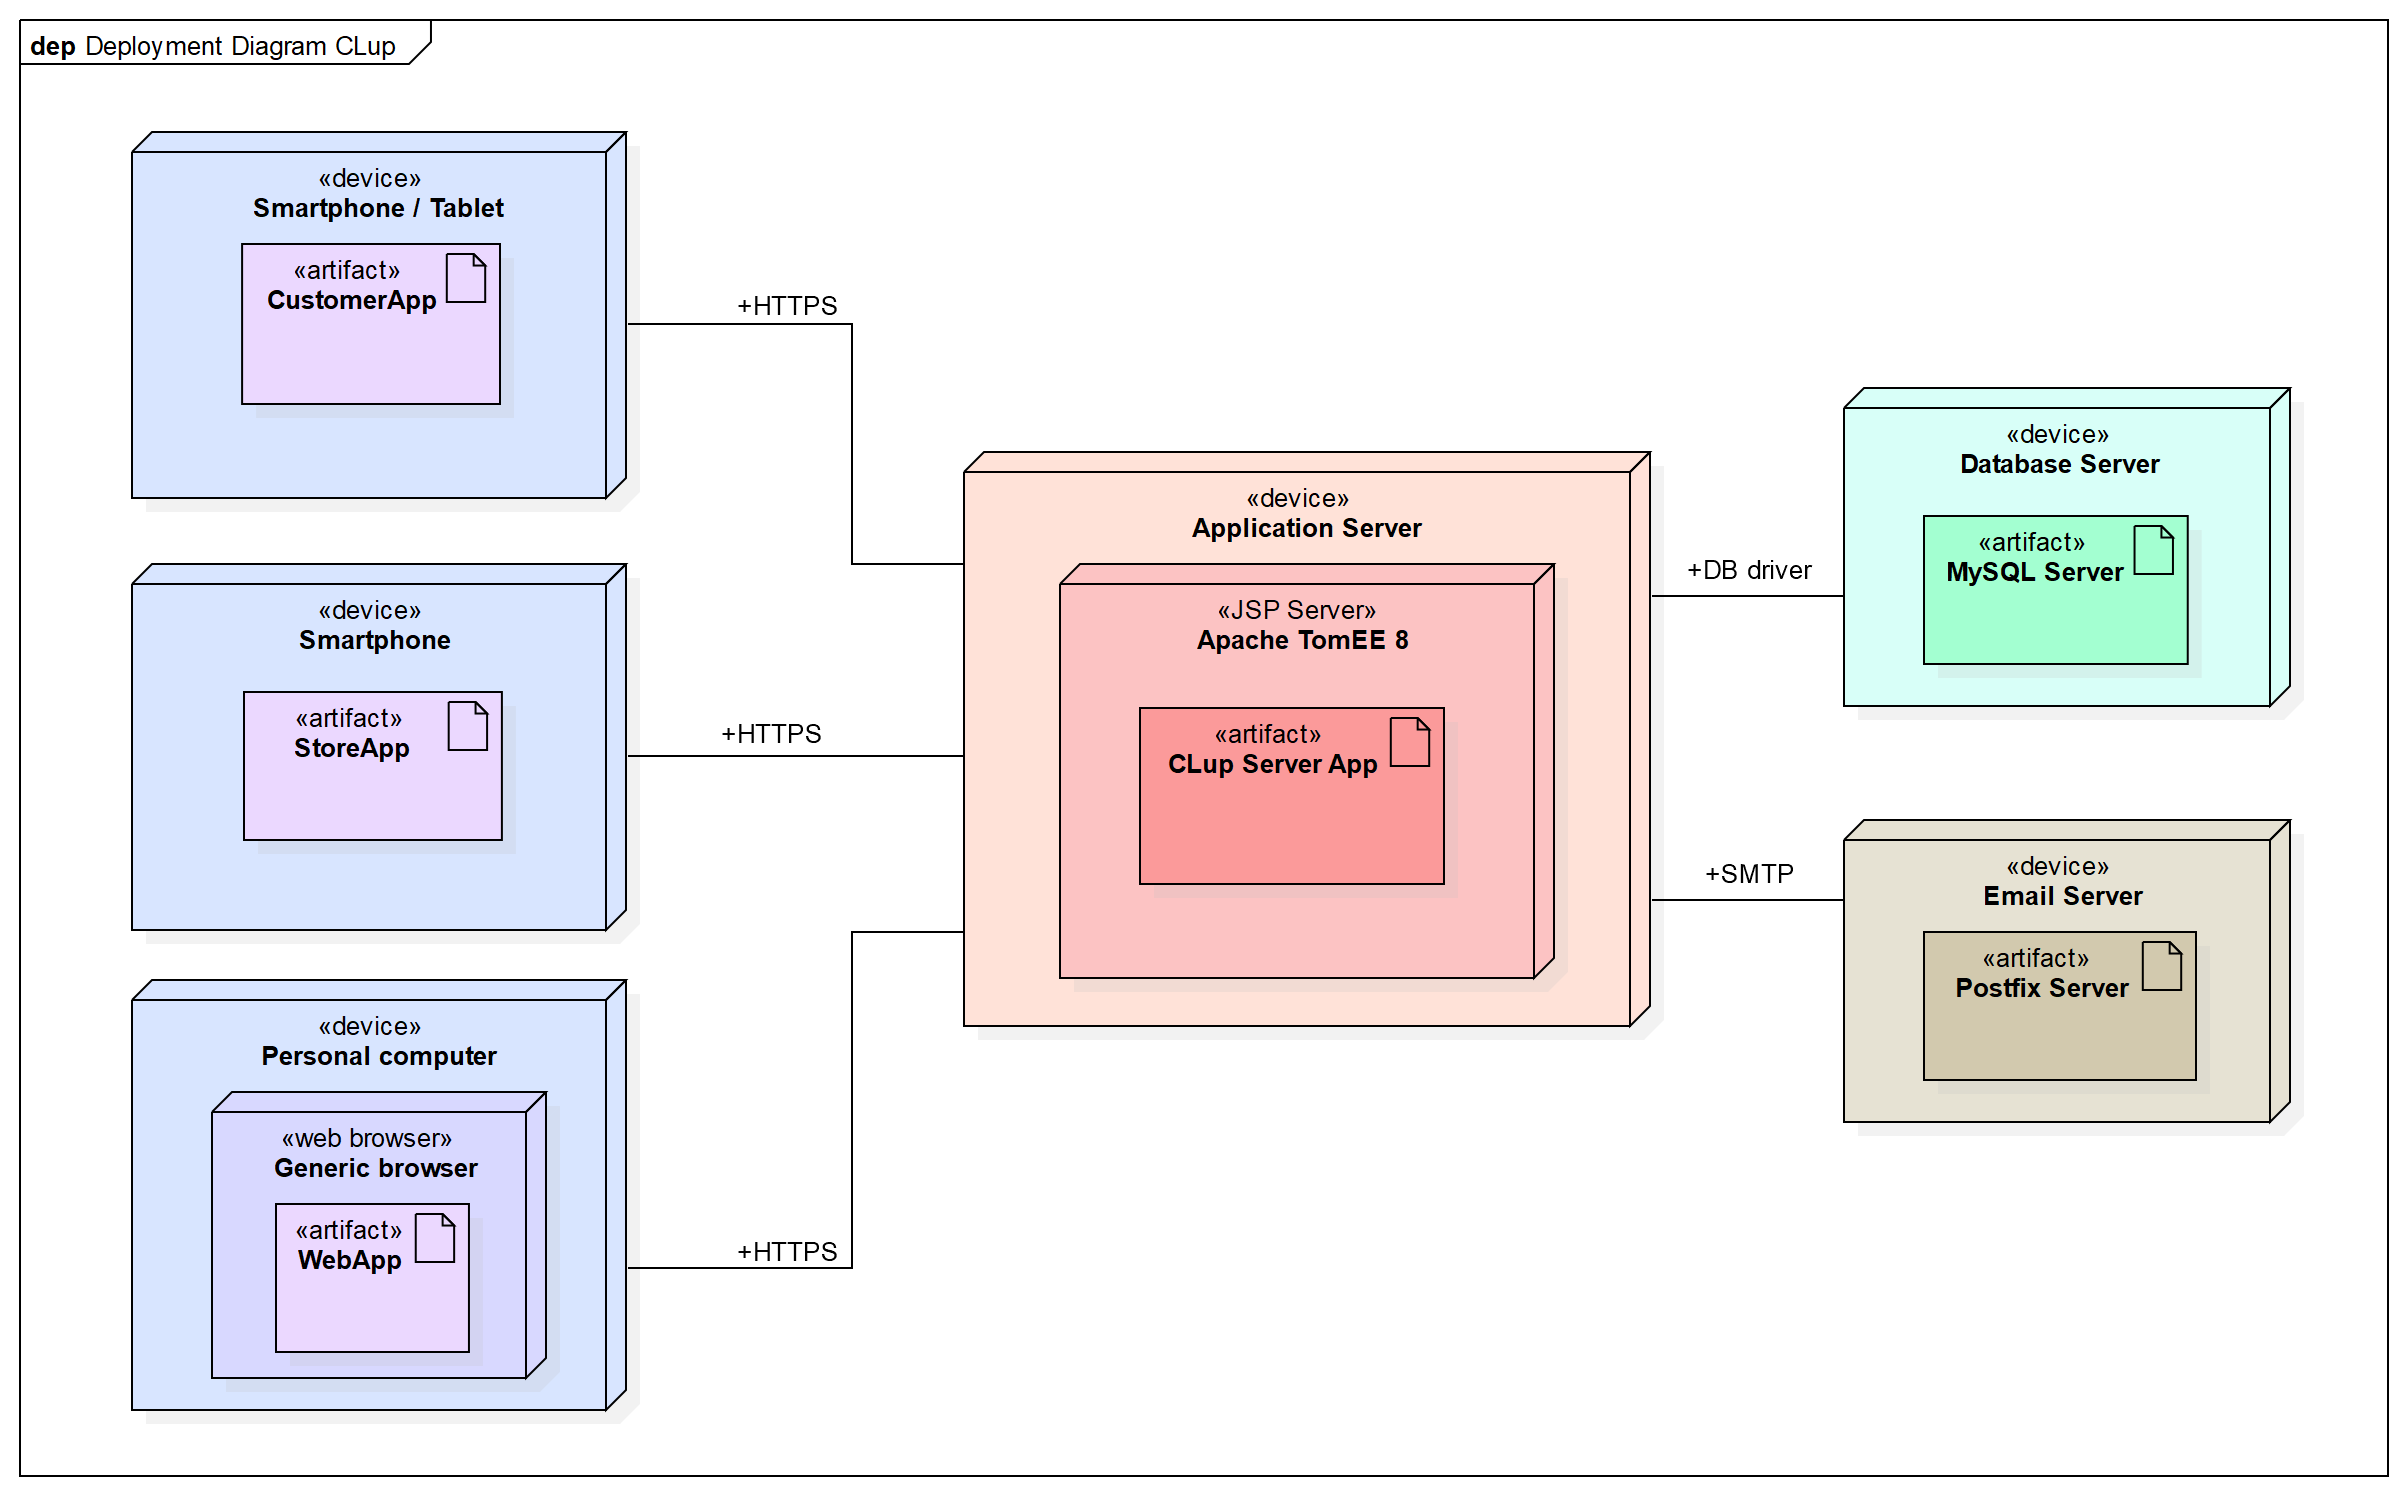
\includegraphics[width=\linewidth]{depl_diag}
	\caption{\textit{Deployment diagram} of the CLup system.}
	\label{fig:depl_diag}
\end{figure}
\clearpage

\section{Runtime view}
This section describes the most important components interactions of the system.\newline
For the sake of simplicity the sequence diagrams are based on the first level of components. 
\subsection{Customer App token}
At the startup, the Customer App will try to request a token to the server via the token manager. Having a token is mandatory in order to take any action with the app.\newline
This process is really important because the token is the only way to identify a customer since no registration is expected. The app will reiterate the process till a valid token is gotten.\newline
This is an automatic process and no action is performed by the user during the operation.
\begin{figure}[H]
	\centering
	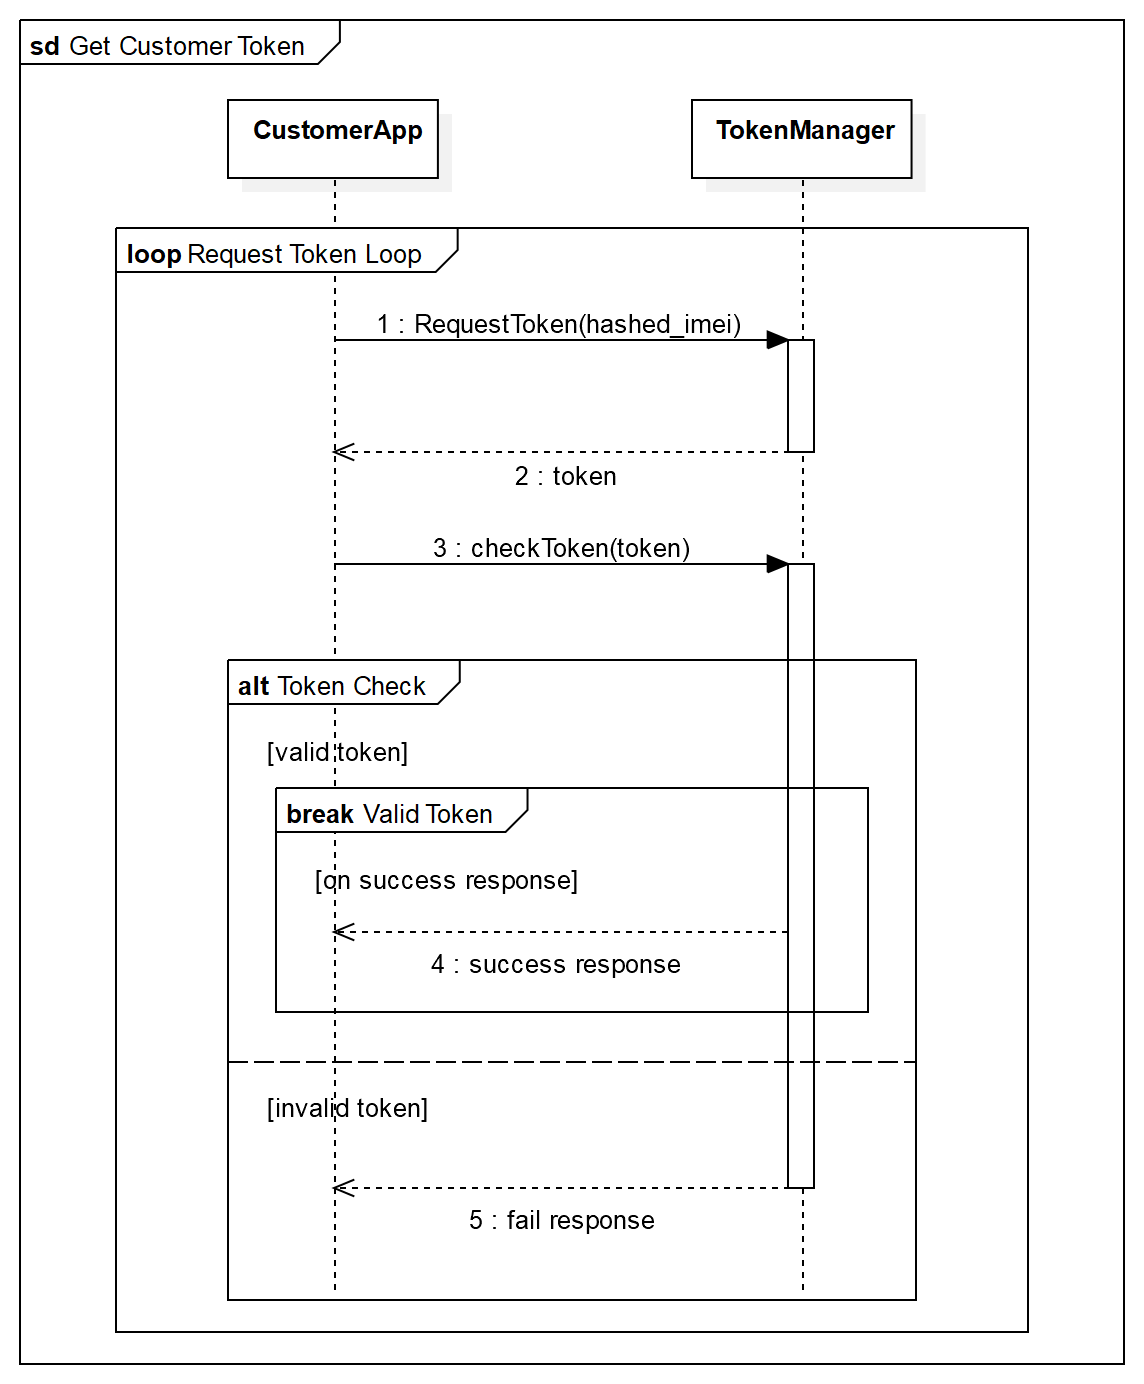
\includegraphics[width=0.8\linewidth]{sequence/seq_token}
	\caption{Customer app token request.}
	\label{fig:seq_token}
\end{figure}
\clearpage

\subsection{Ticket request}
The request for a ticket starts from the Customer App and contains both token and selected store. The token validation is the first operation performed by the server and consequently, if all the checks go well, a ticket is retrieved.
\vspace{0.1cm}
\begin{figure}[H]
	\centering
	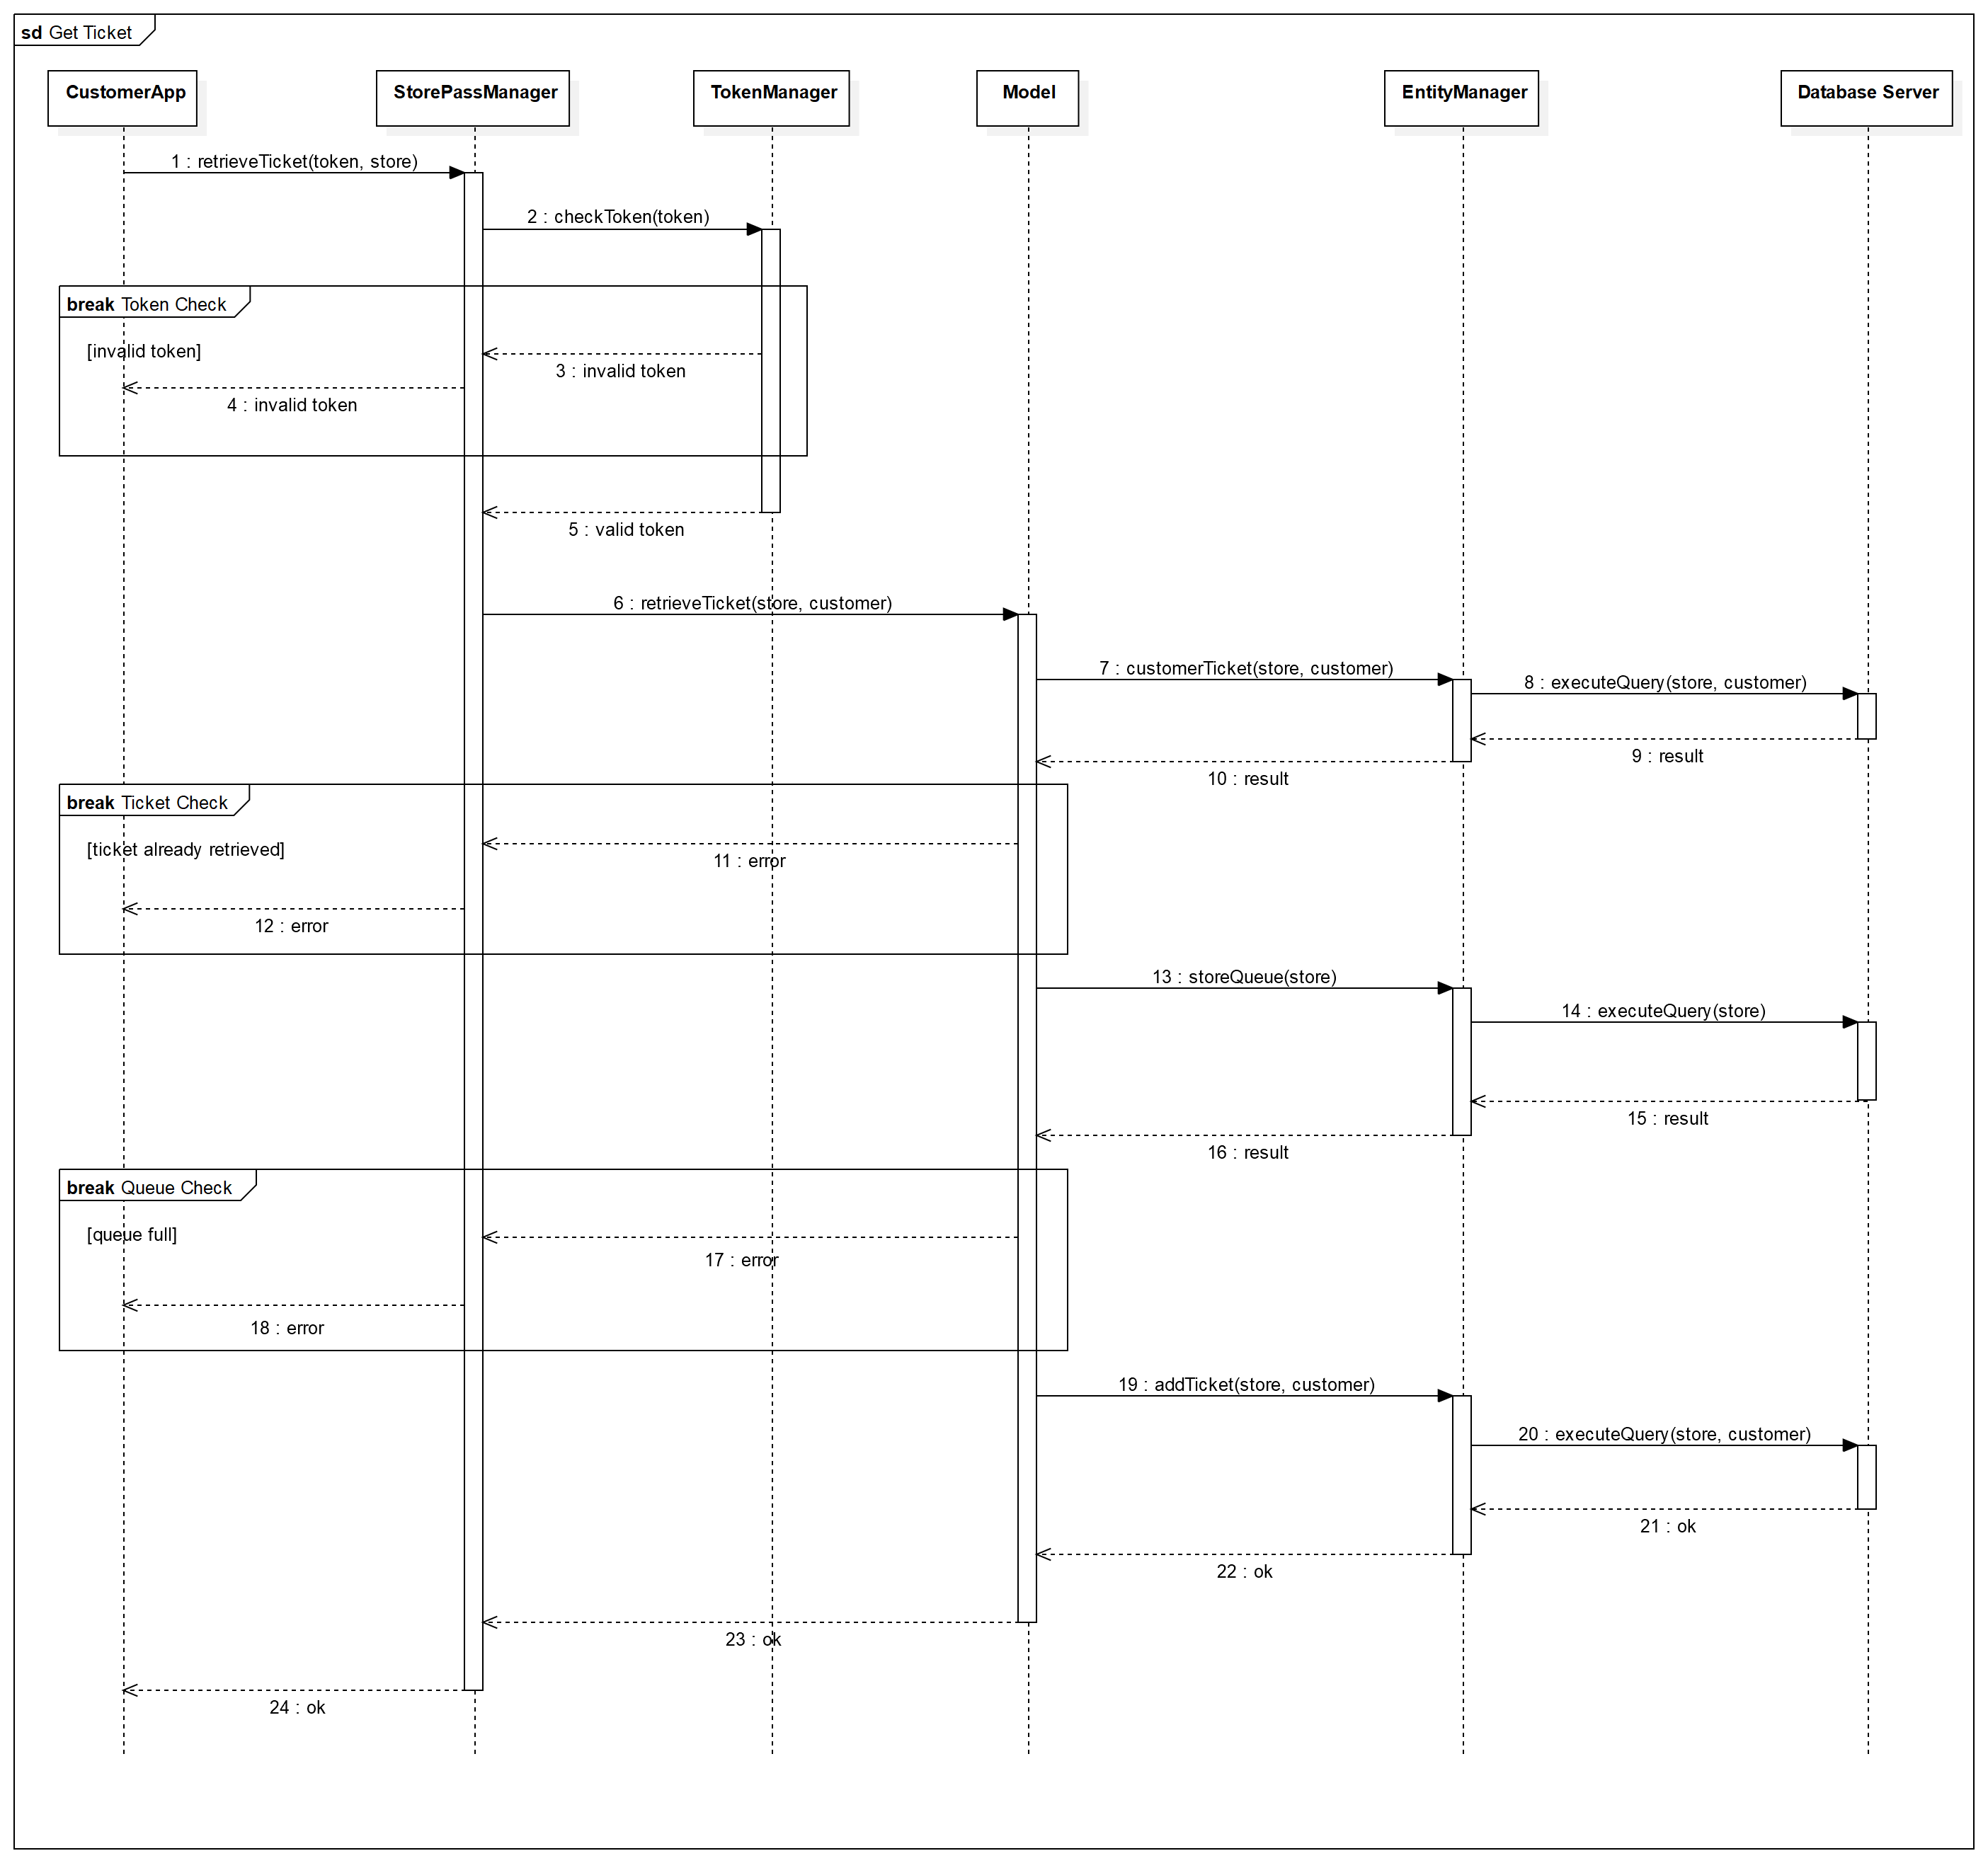
\includegraphics[width=\linewidth]{sequence/seq_ticket}
	\caption{Ticket request.}
	\label{fig:seq_ticket}
\end{figure}

\clearpage

\subsection{Booking request}
A user can book a visit for a store if he hasn't booked a visit to the same store and in the same day yet. This check is done together with the token validation and others checks.\newline
Since a booking must be confirmed via a link, an email is sent at the end of the whole process through the mail server.
\begin{figure}[H]
	\centering
	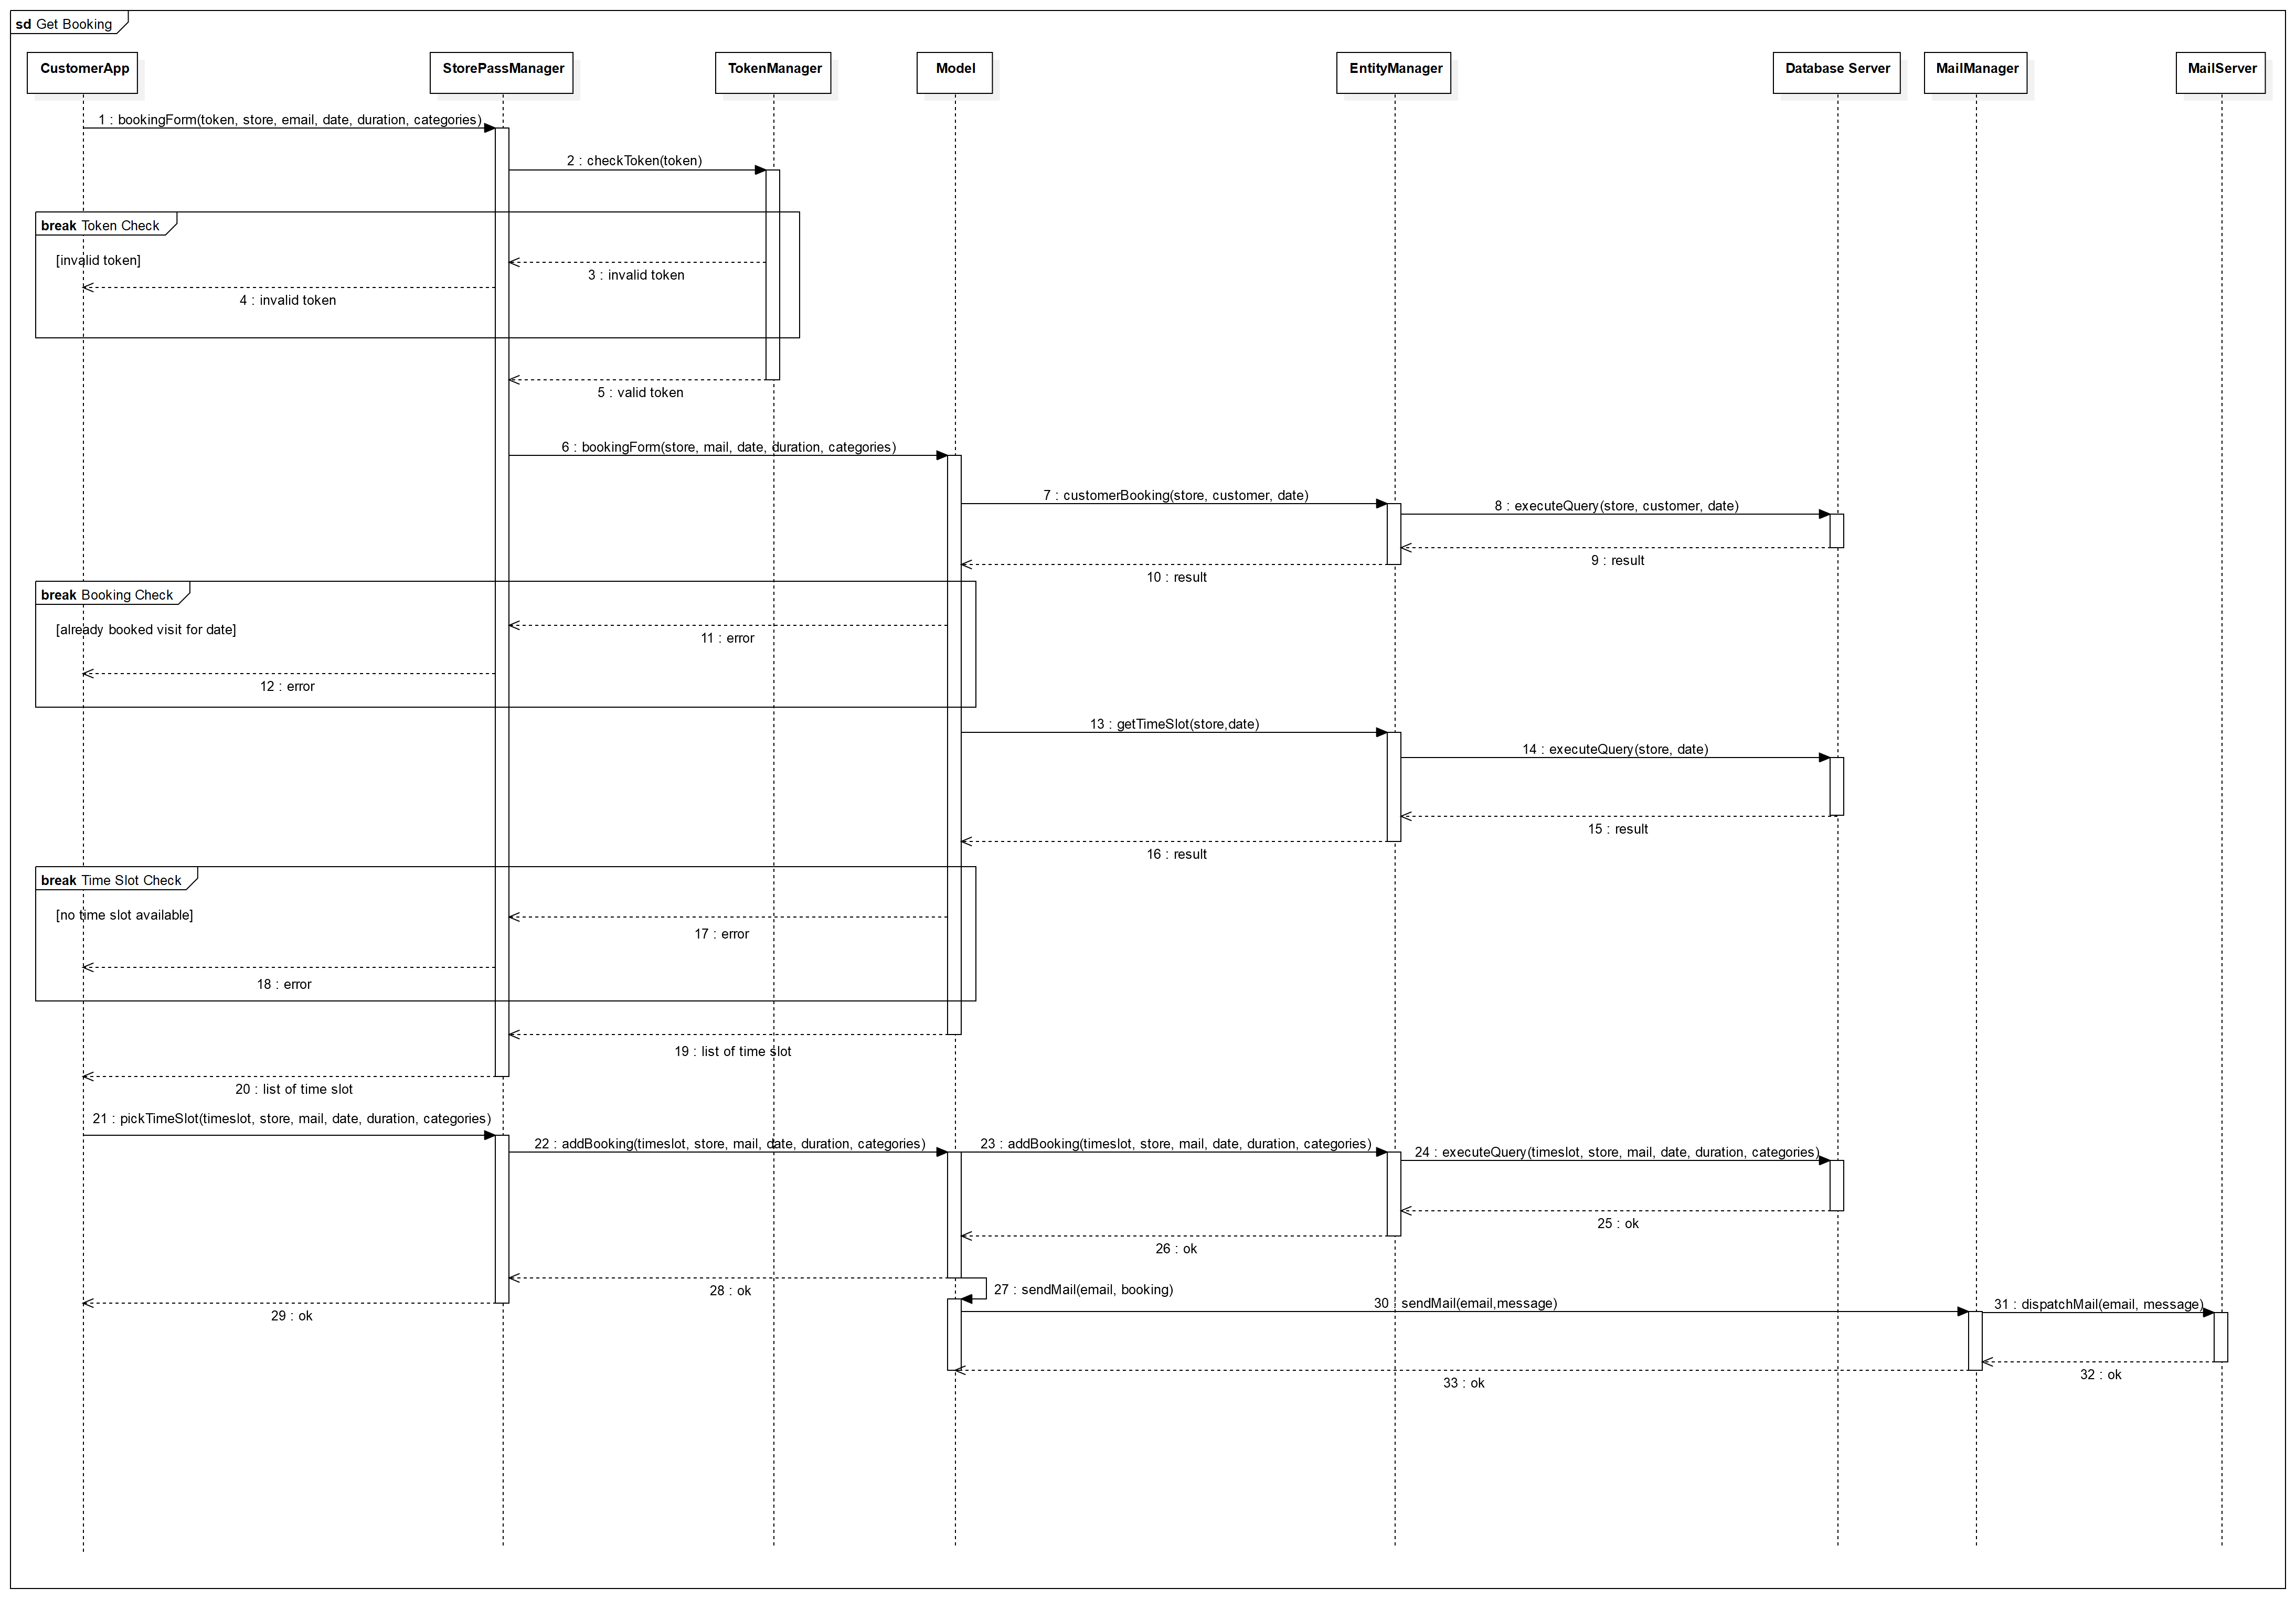
\includegraphics[angle=90,origin=c,height=\linewidth]{sequence/seq_booking}
	\caption{Booking request.}
	\label{fig:seq_booking}
\end{figure}

\clearpage
\subsection{Leave At Time}
The Customer App reminds the user to leave the place where he is in order to ensure that he arrives on time.\newline
The server fetches all the valid store passes and computes the distance of the customer from the respective store. If the customer should leave the place where he is, a notification is sent to him.
\begin{figure}[H]
	\centering
	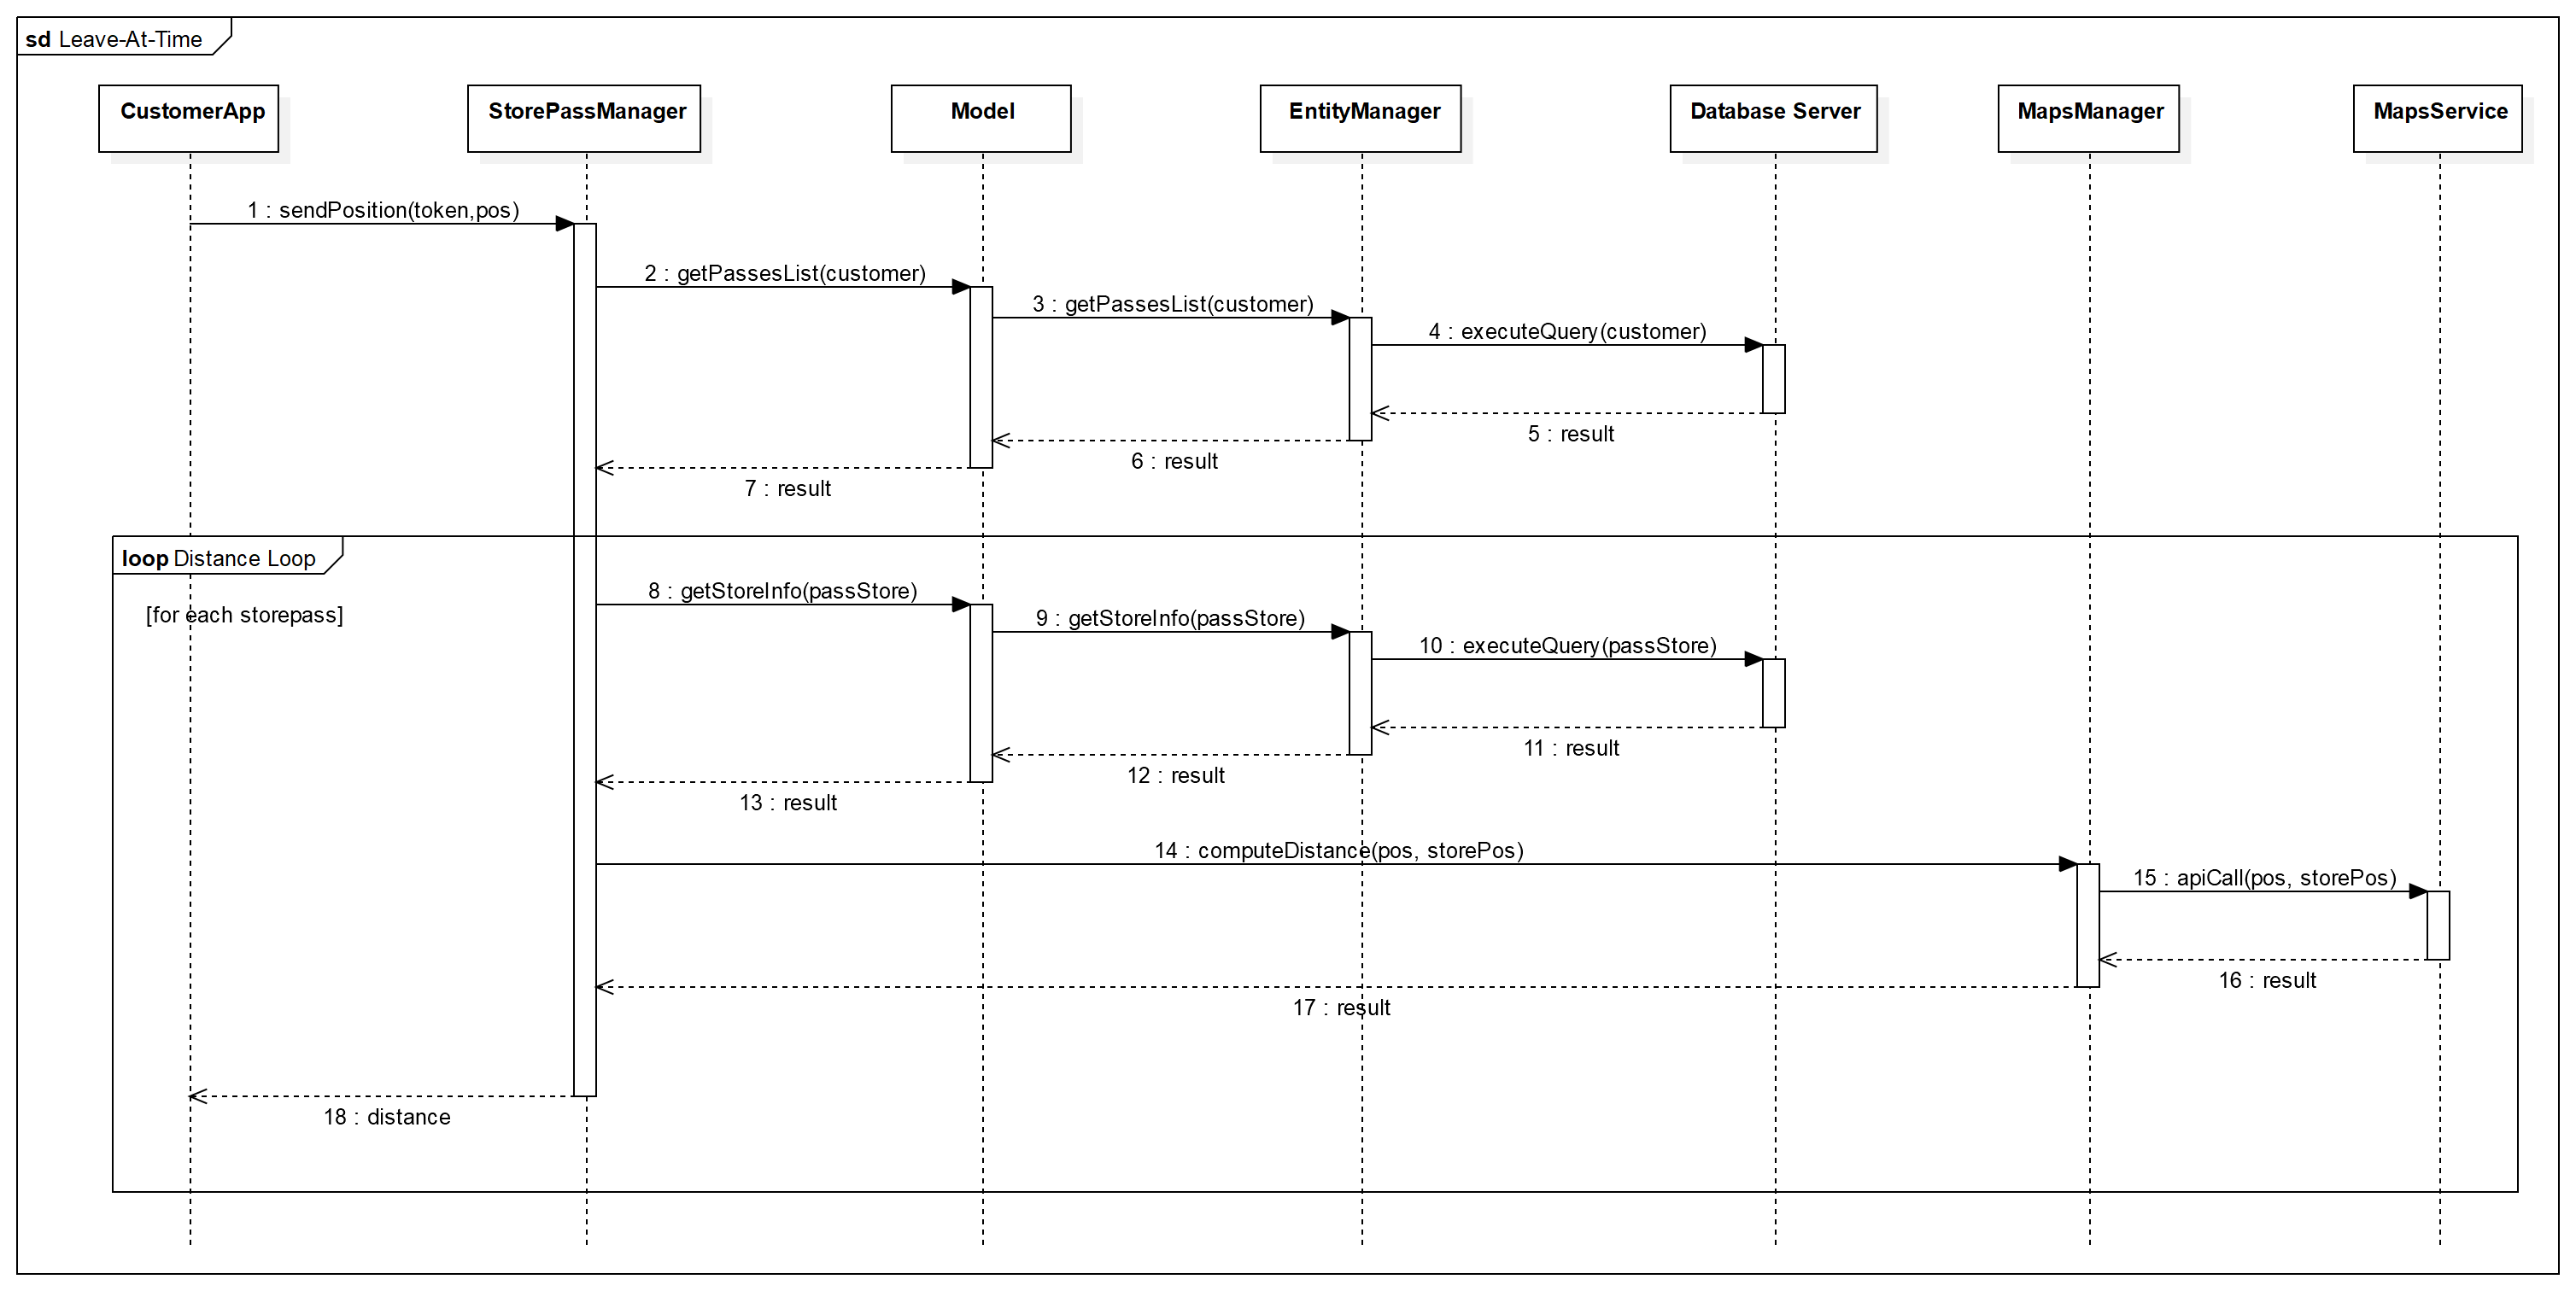
\includegraphics[width=0.75\linewidth]{sequence/seq_leave}
	\caption{Leave at time function.}
	\label{fig:seq_leave}
\end{figure}

\subsection{Web App login}
The following sequence diagram represents the login process to the Web App. CLup admins, store managers and store employees will authenticate to the system by submitting their credentials via a form.
\begin{figure}[H]
	\centering
	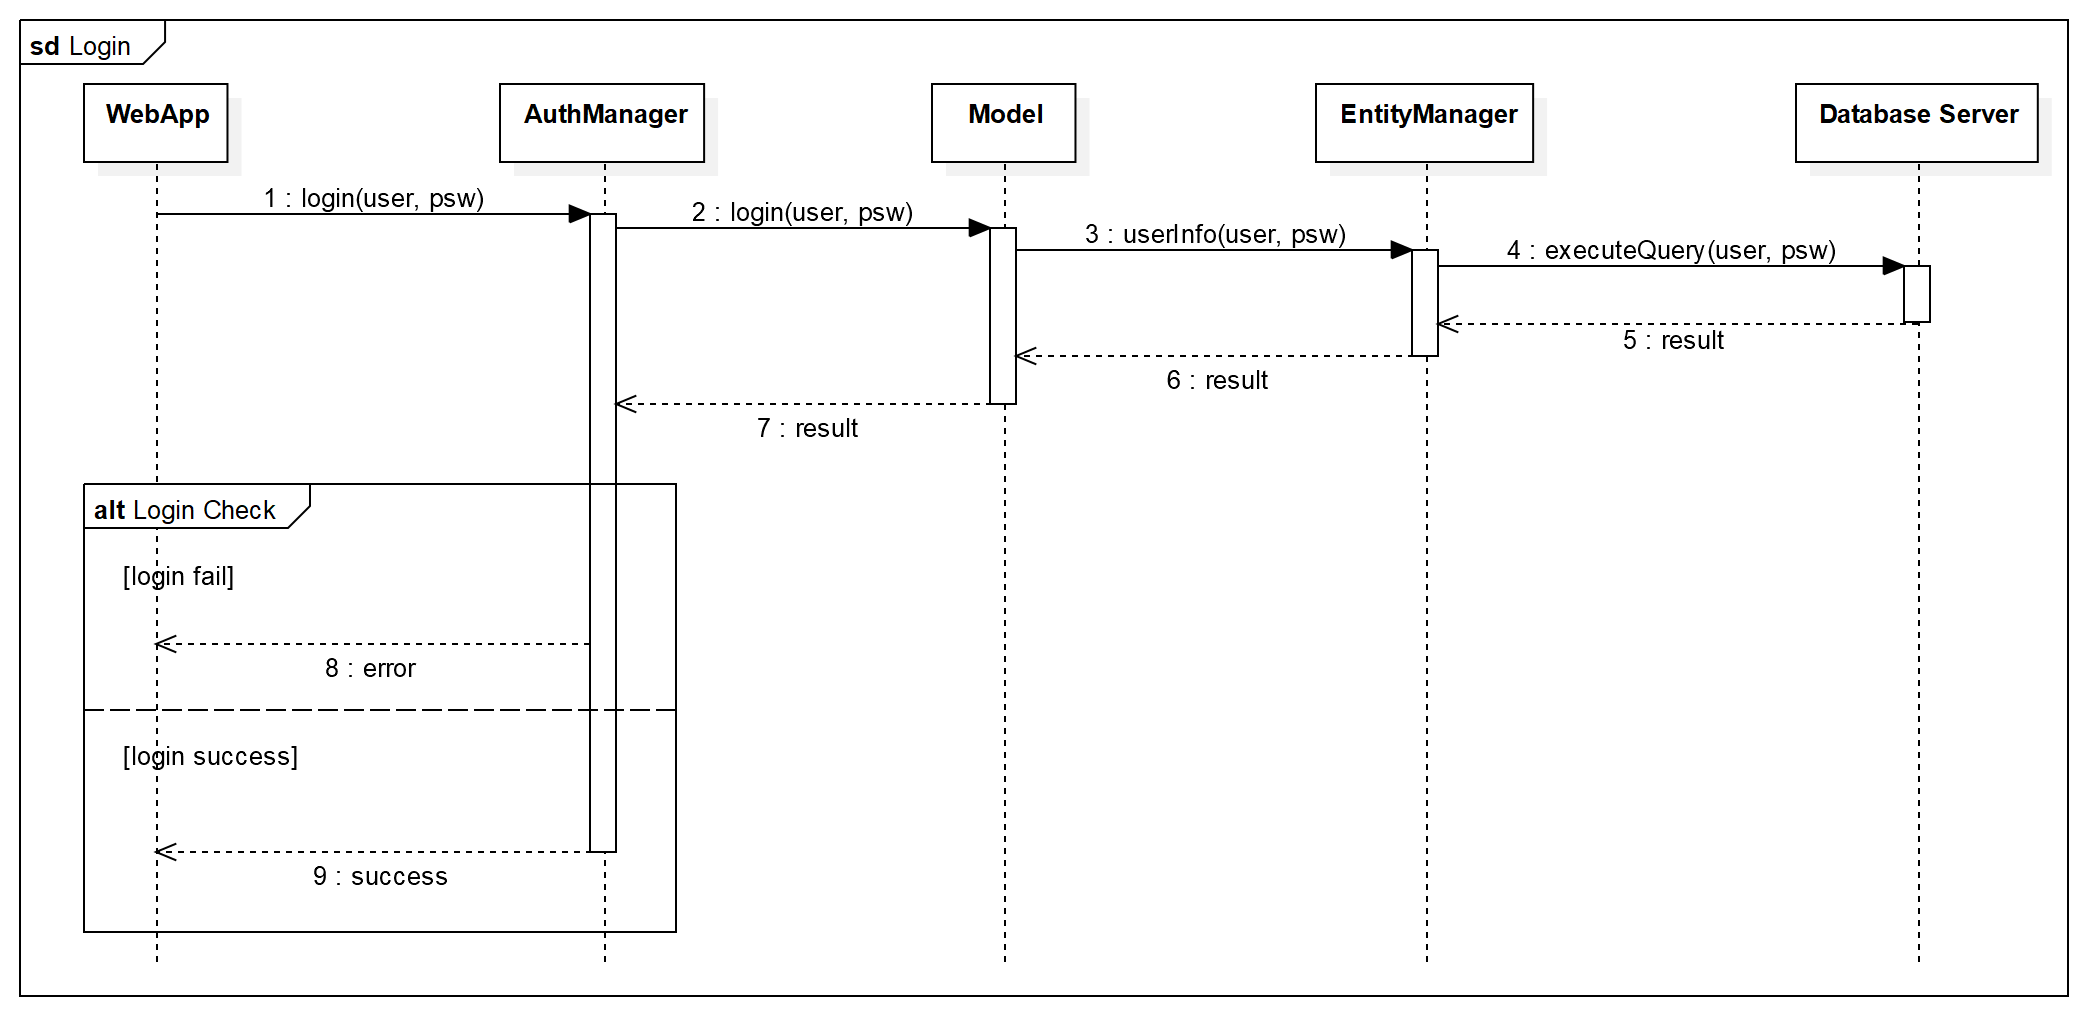
\includegraphics[width=0.75\linewidth]{sequence/seq_login}
	\caption{Web App login.}
	\label{fig:seq_login}
\end{figure}

\subsection{Check store status}
After logging in, the store managers can see the store status, for instance the visits booked. The following sequence diagram represents this process. 
\begin{figure}[H]
	\centering
	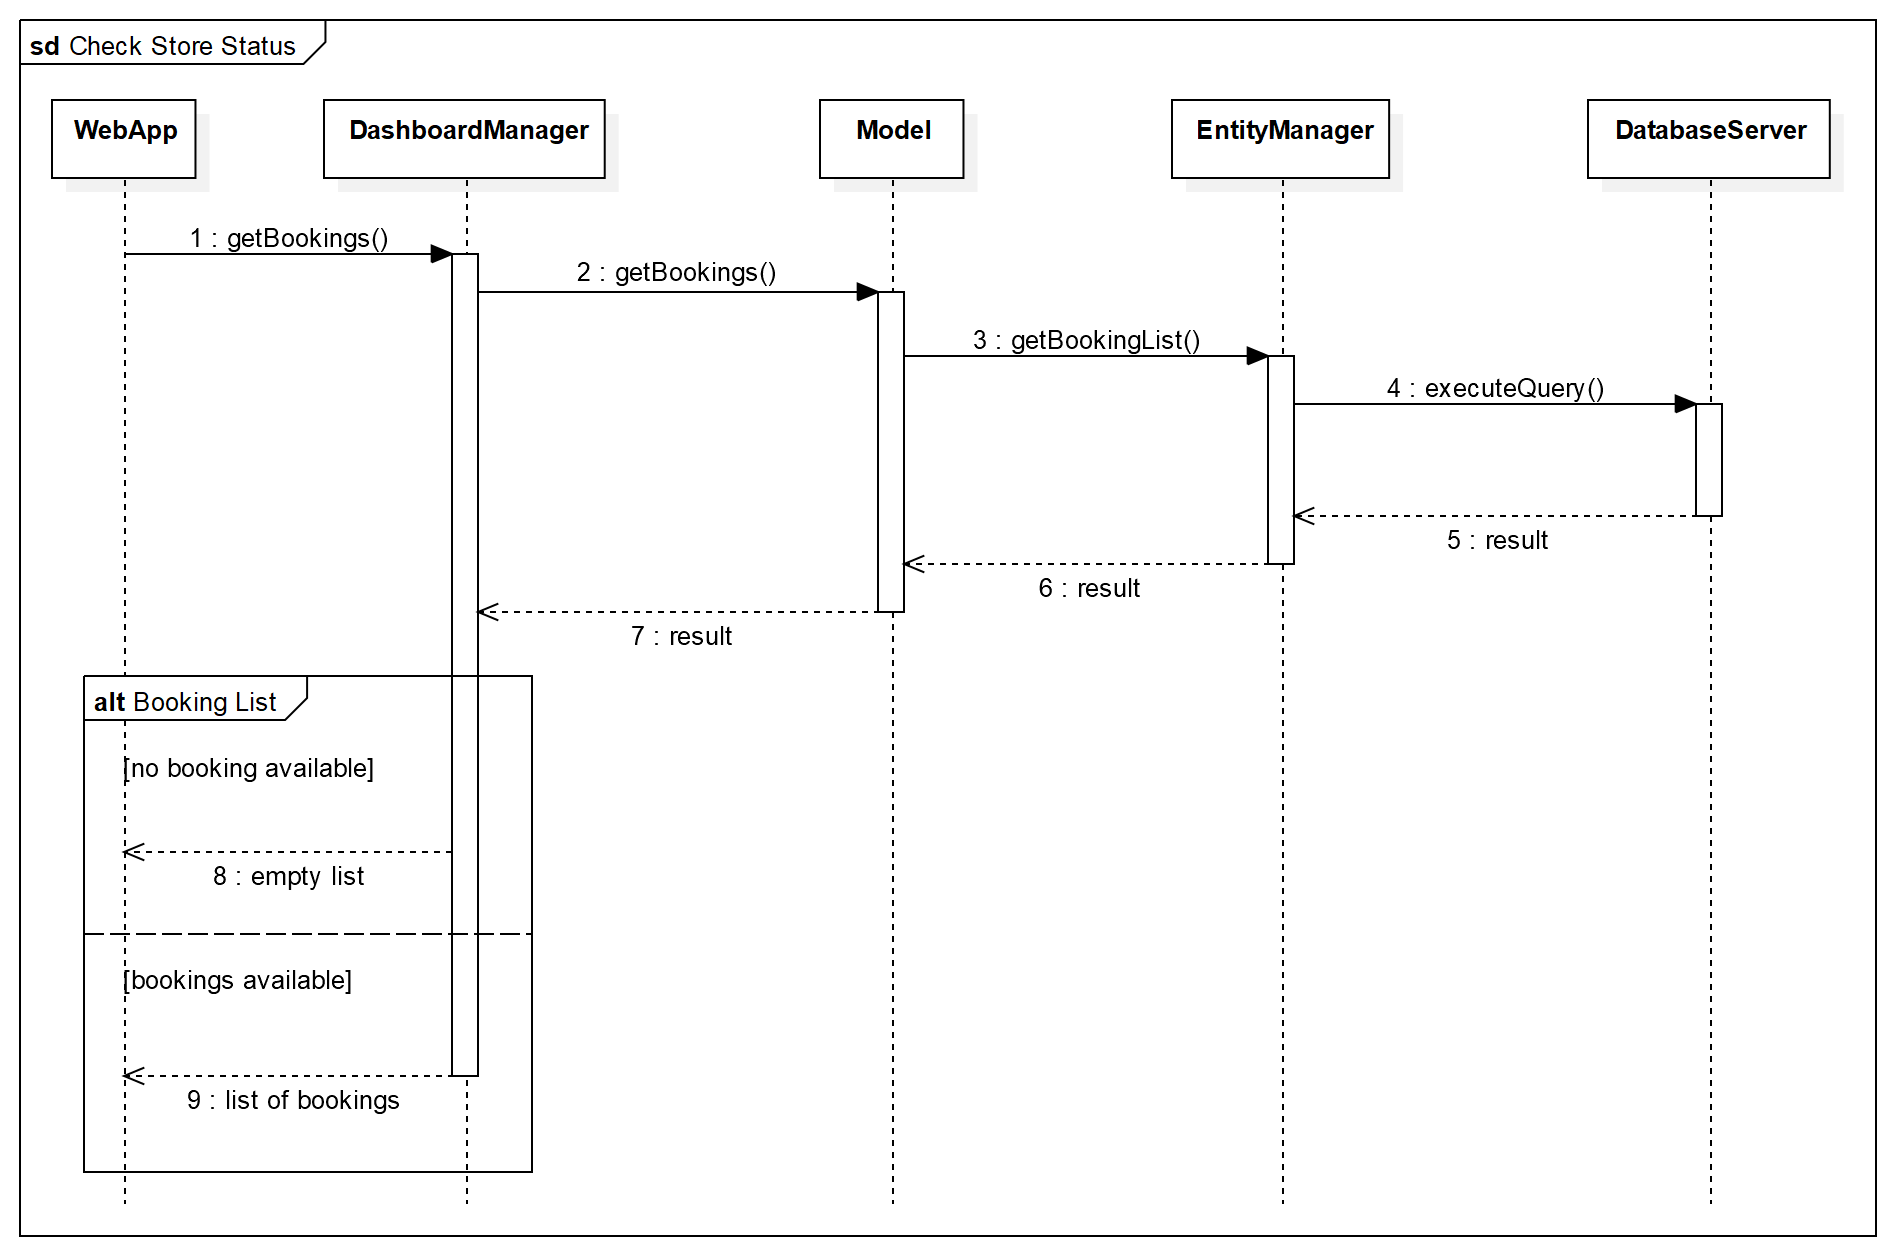
\includegraphics[width=0.75\linewidth]{sequence/seq_check_status}
	\caption{Check store status.}
	\label{fig:seq_check_status}
\end{figure}

\subsection{Store App login}
As the Customer App, Store App also has a token to operate. This time there is a login process before the generation of the token.
\begin{figure}[H]
	\centering
	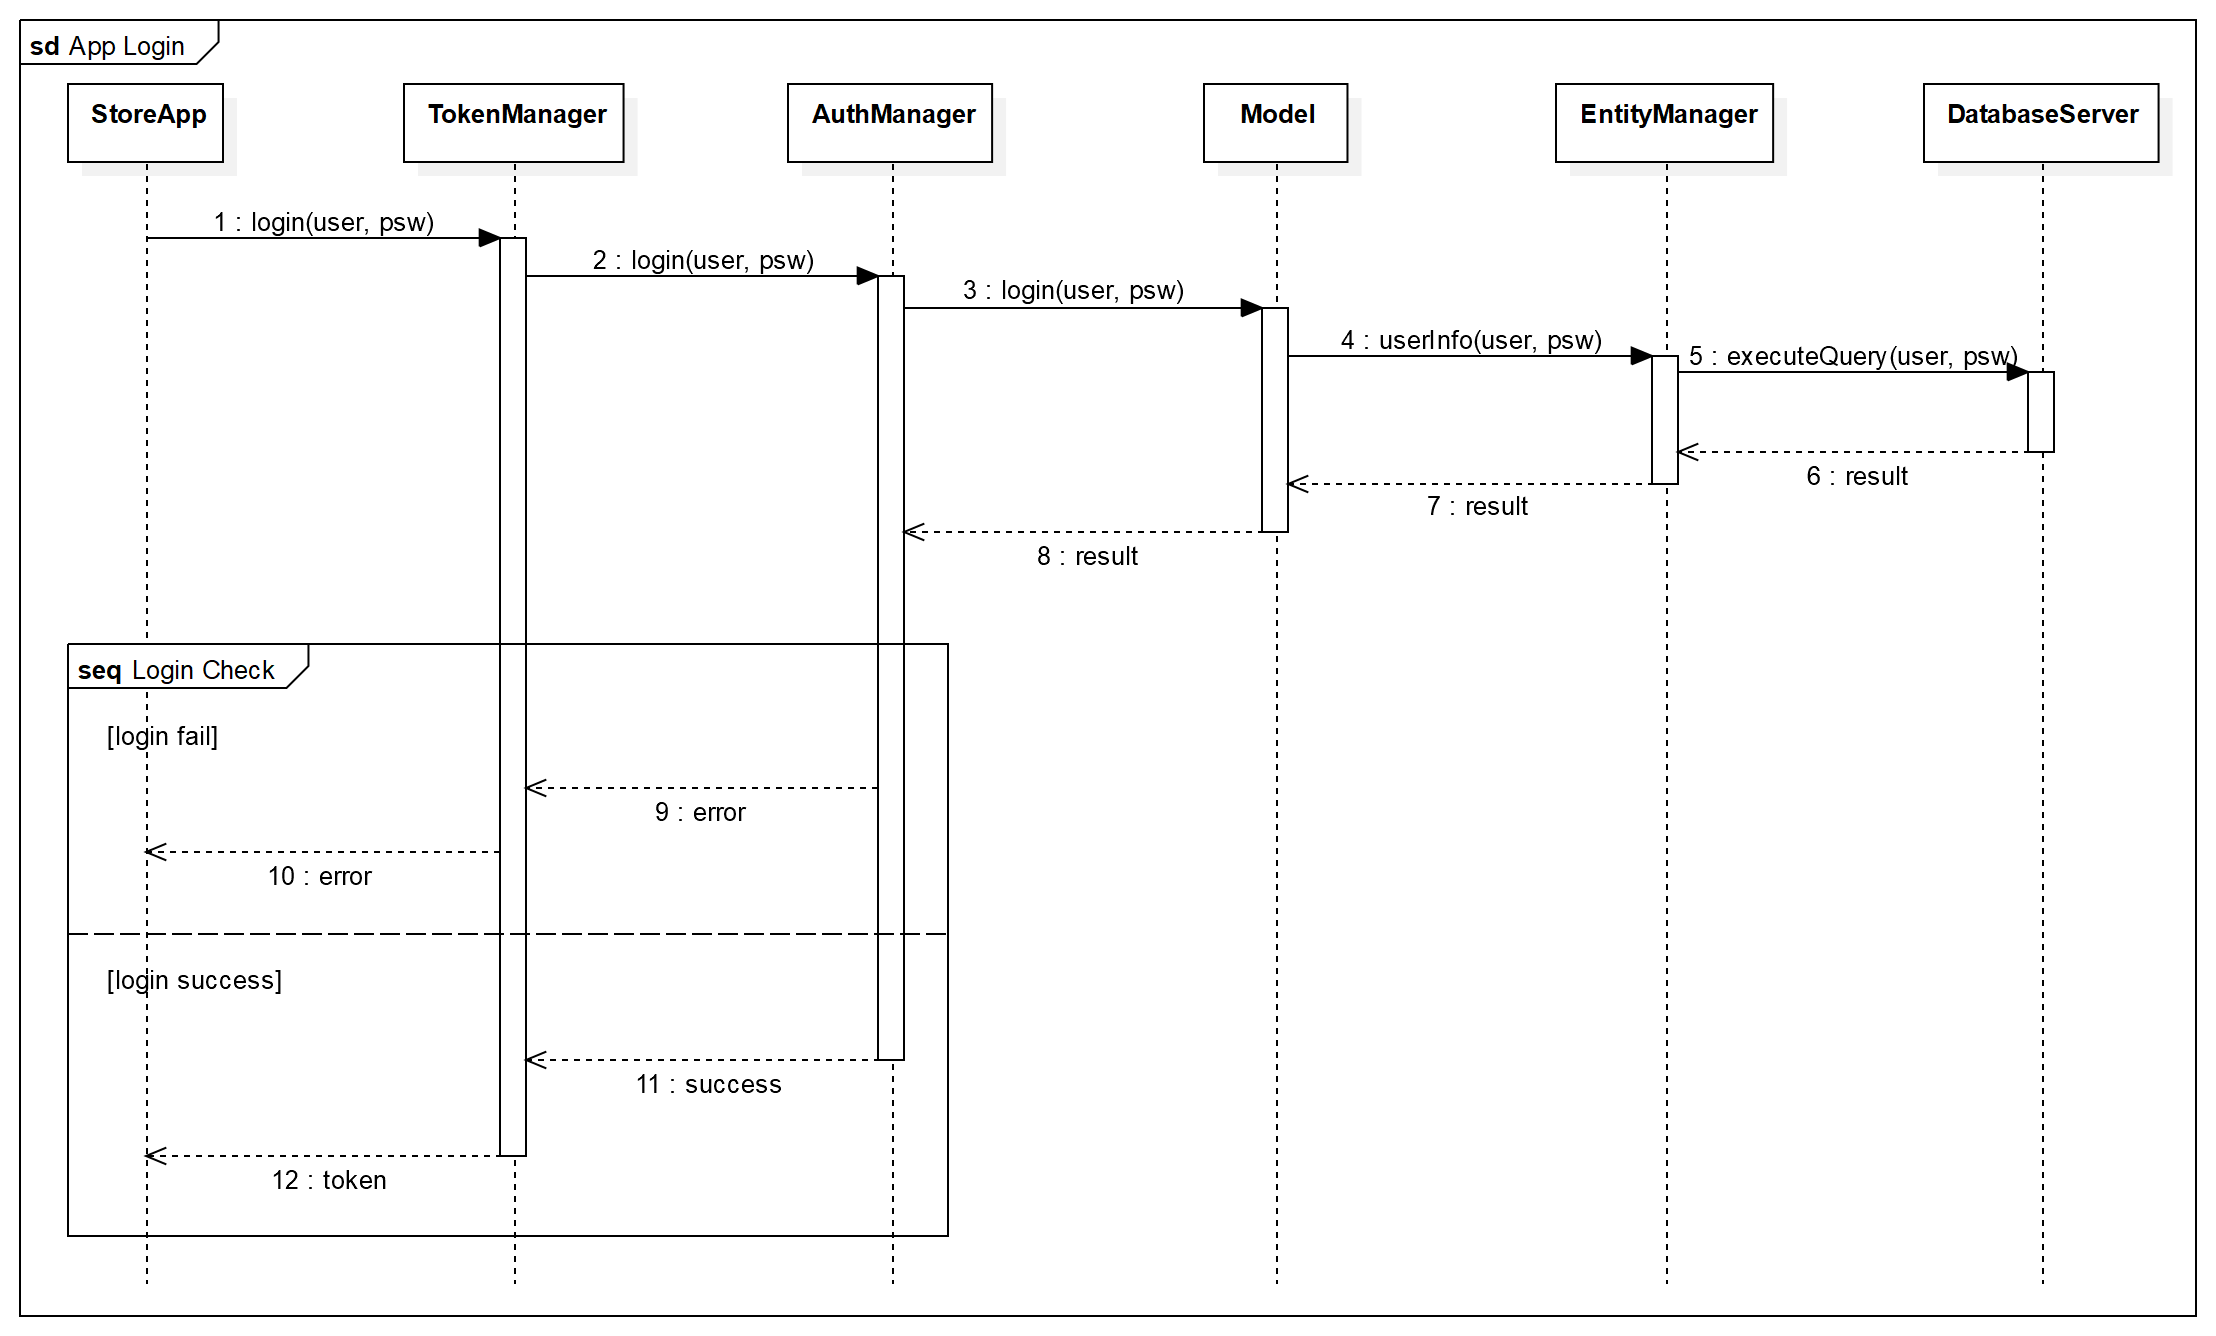
\includegraphics[width=0.75\linewidth]{sequence/seq_app_login}
	\caption{Store app login.}
	\label{fig:seq_app_login}
\end{figure}

\subsection{QR Code scan}
The scan of the QR is the most important part of the Store App. After the token validation, the QR code is validated as the sequence diagram shows. If the pass is valid, his status is updated.
\begin{figure}[H]
	\centering
	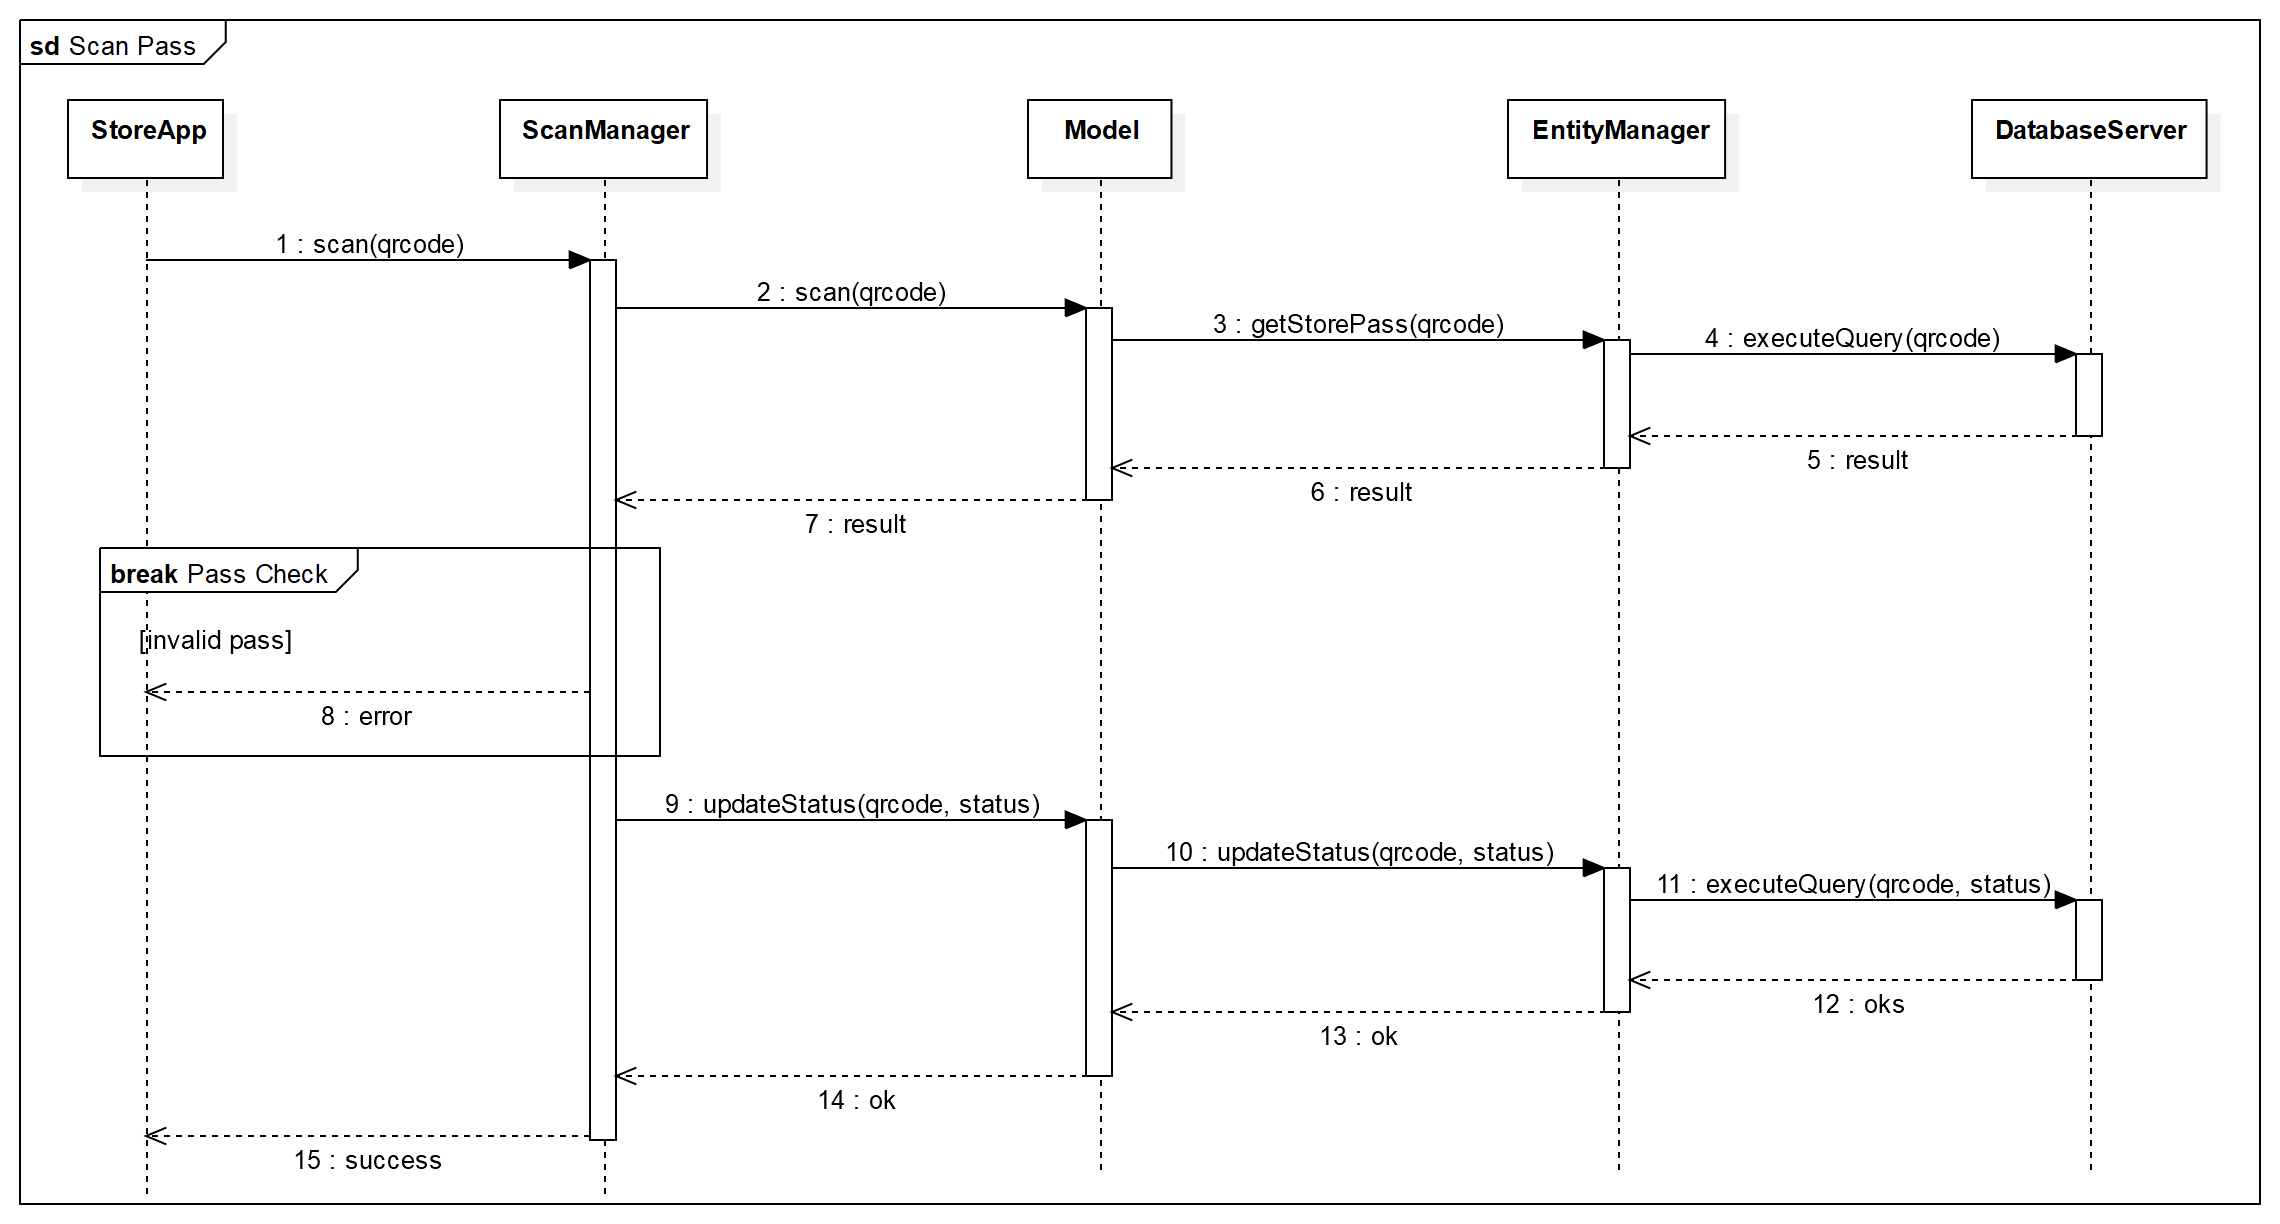
\includegraphics[width=0.85\linewidth]{sequence/seq_scan_pass}
	\caption{Store app scan process.}
	\label{fig:seq_scan_pass}
\end{figure}

\subsection{Store registration}
The store registration is performed by a CLup admin via the Web App after his login. Prompted informations are checked from the system and then, if the store doesn't already exist, the store is saved into the database. After that, the credentials for the store managers and store employees are generated and sent to the store PEC address.
\begin{figure}[H]
	\centering
	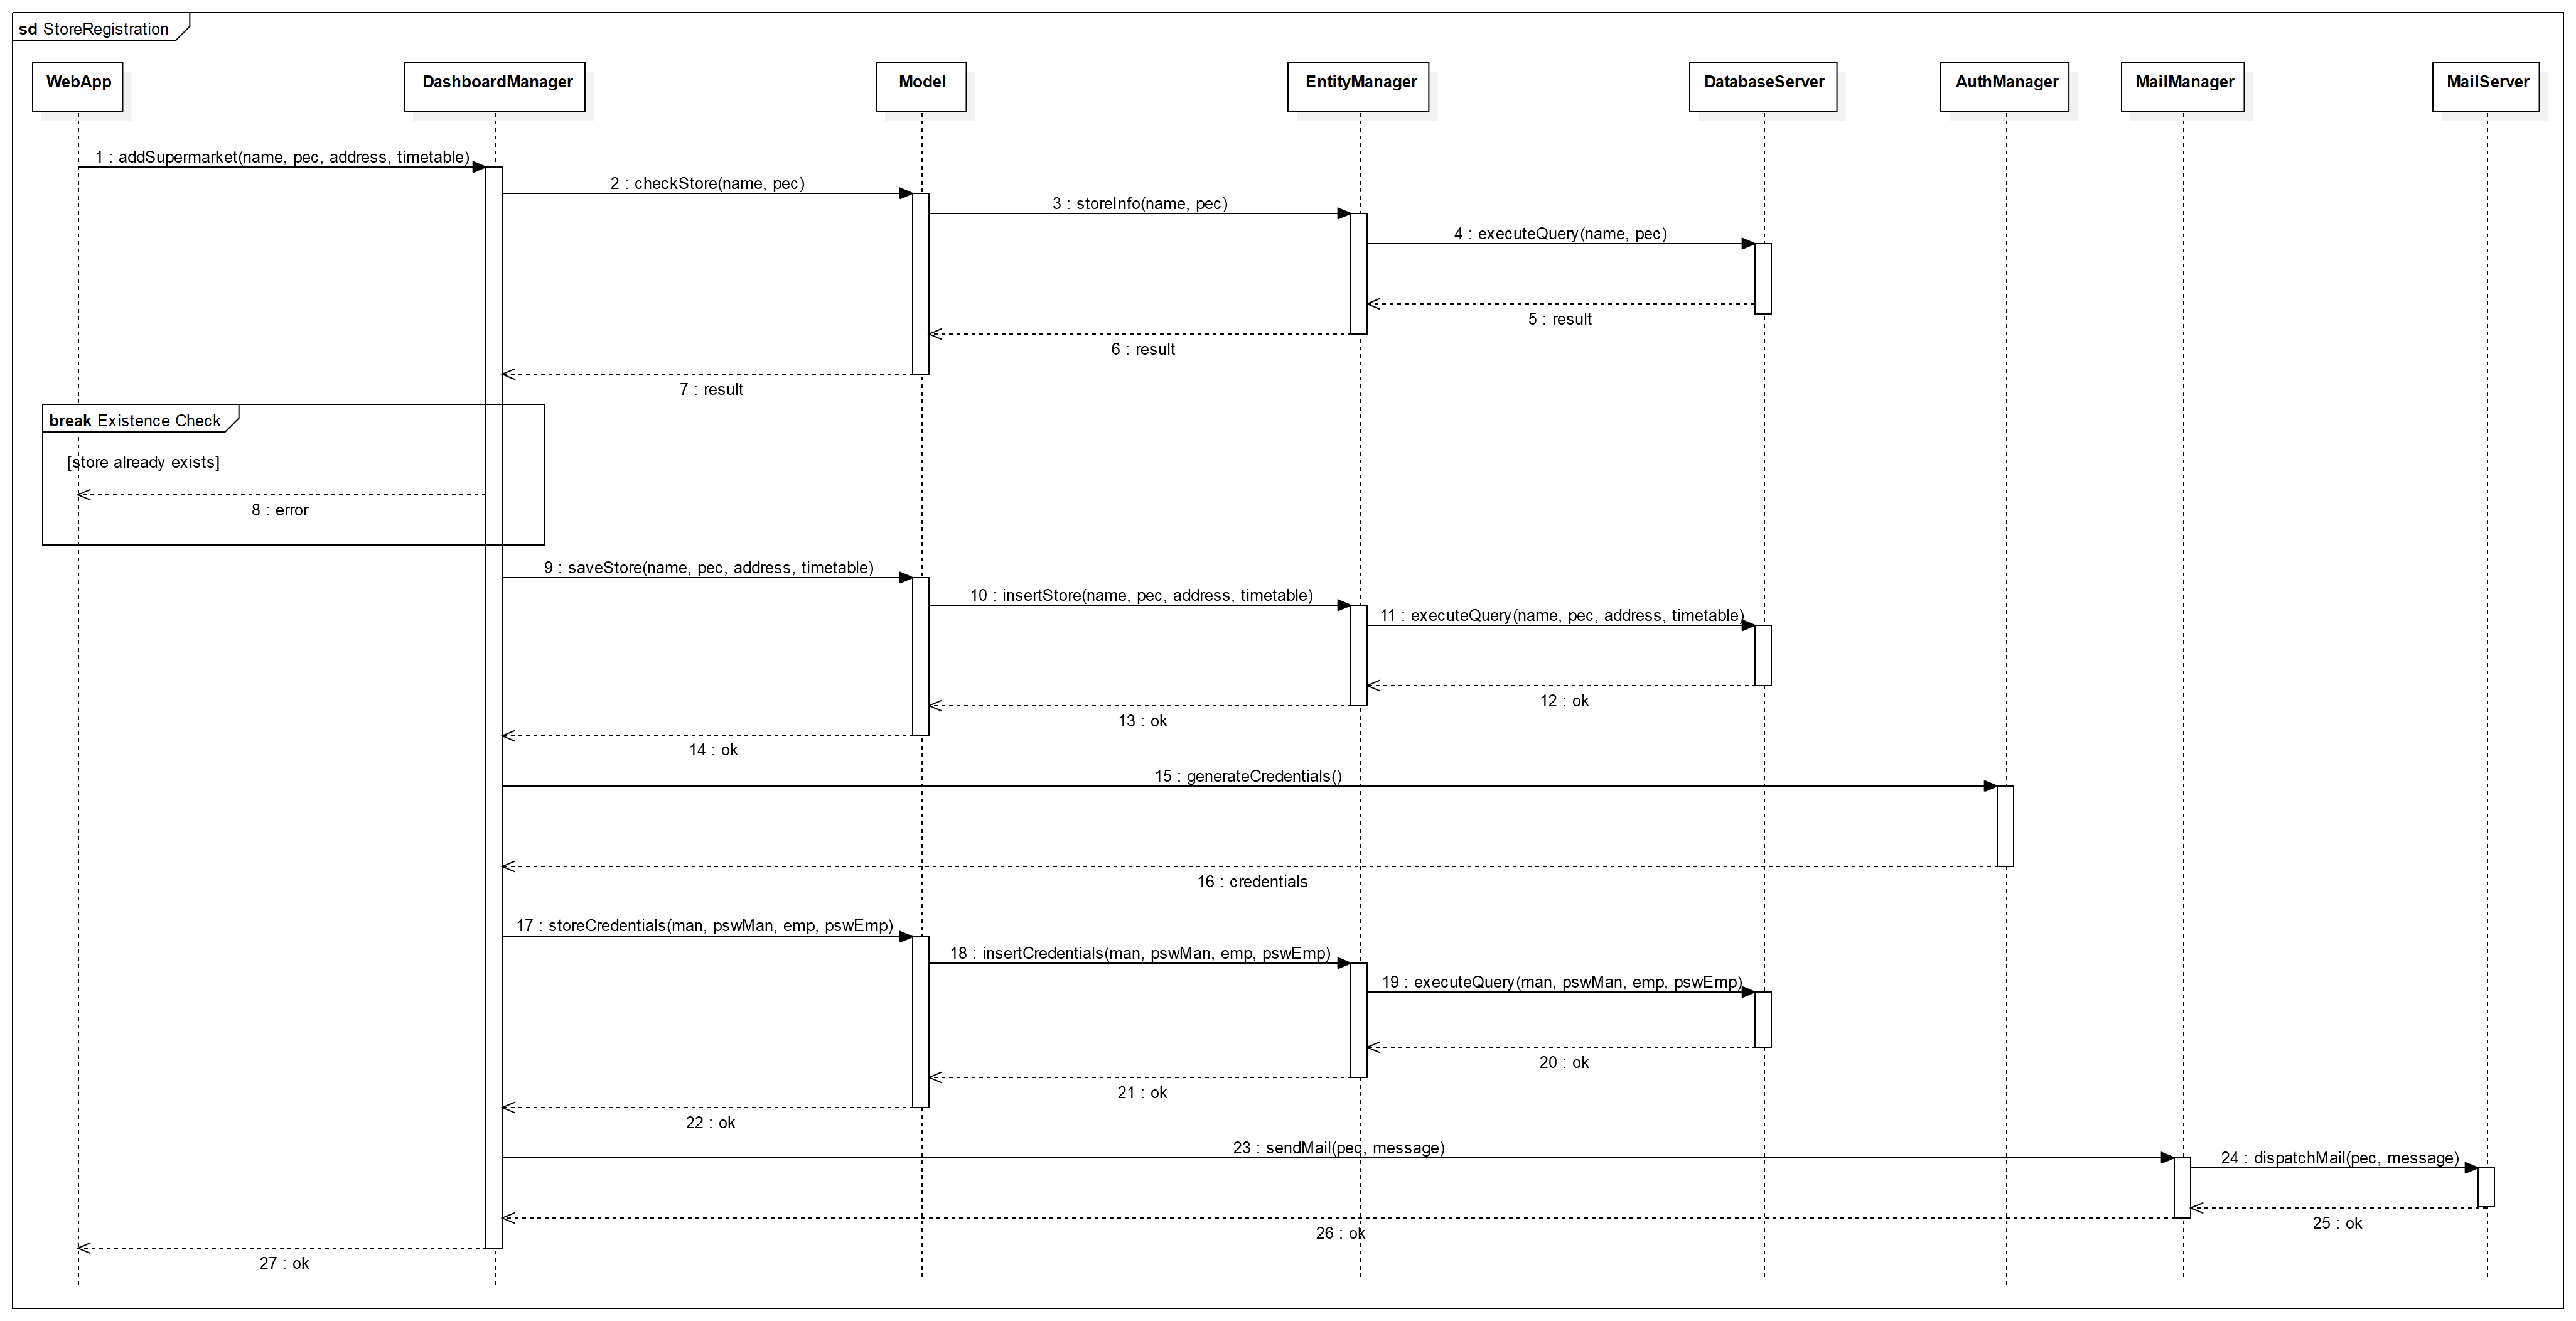
\includegraphics[width=0.85\linewidth]{sequence/seq_store_registration}
	\caption{Store registration.}
	\label{fig:seq_store_registration}
\end{figure}

\section{Component interfaces}
This section lists all the methods that each component interface provides to the other components.

\begin{itemize}
	\item \textbf{ViewInfoInterface}
	\begin{itemize}
		\item getStores(token, filters)
		\item getStoreInfo(token, store)
	\end{itemize}

	
	\item \textbf{StorePassInterface}
	\begin{itemize}
		\item retrieveTicket(token, store)
		\item bookingForm(token, store, email, date, duration, categories)
		\item pickTimeSlot(timeslot, store, mail, date, duration, categories)
		\item getPassesList(token)
		\item getPassInfo(token, pass)
		\item deletePass(token, pass)
	\end{itemize}

	\item \textbf{ScanInterface}
	\begin{itemize}
		\item scan(qrcode)
	\end{itemize}
	
	\item \textbf{TokenInterface}
	\begin{itemize}
		\item requestToken()
		\item checkToken(token)
		\item login(user, psw)
	\end{itemize}

	\item \textbf{AuthInterface}
	\begin{itemize}
		\item login(user, psw)
	\end{itemize}

	\item \textbf{DashboardInterface}
	\begin{itemize}
		\item getStoreStatus()
		\item getTickets()
		\item getBookings()
		\item deletePass(pass)
		\item updateStoreInfo(info)
		\item addSupermarket(name, pec, address, timetable)
		\item regenerateCredentials(store)
	\end{itemize}

	\item \textbf{TokenAuthInterface}
	\begin{itemize}
		\item login(user, psw)
	\end{itemize}

	\item \textbf{AuthCredentialsInterface}
	\begin{itemize}
		\item generateCredentials()
	\end{itemize}

	\item \textbf{TokenCheckInterface}
	\begin{itemize}
		\item checkToken(token)
	\end{itemize}

	\item \textbf{MailManagerInterface}
	\begin{itemize}
		\item sendMail(email, message)
	\end{itemize}

	\item \textbf{ModelInterface}
	\begin{itemize}
		\item retrieveTicket(store, customer)
		\item bookingForm(store, mail, date, duration, categories)
		\item addBooking(timeslot, store, mail, date, duration, categories)
		\item login(user, psw)
		\item getBookings()
		\item scan(qrcode)
		\item updateStatus(qrcode, status)
		\item checkStore(name, pec)
		\item saveStore(name, pec, address, timetable)
		\item storeCredentials(man, pswMan, emp, pswEmp)
		\item updateCredentials(store, man, pswMan, emp, pswEmp)
		\item getStores(filters)
		\item getStoreInfo(store)
		\item getPassesList(customer)
		\item getPassInfo(pass)
		\item deletePass(pass)
		\item getStoreStatus()
		\item getTickets()
		\item deletePass(pass)
		\item updateStoreInfo(info)
	\end{itemize}

	\item \textbf{EntityManagerInterface}
	\begin{itemize}
		\item getCustomerTicket(store, customer)
		\item getStoreQueue(store)
		\item addTicket(store, customer)
		\item getCustomerBooking(store, customer, date)
		\item getTimeSlot(store, date)
		\item addBooking(timeslot, store, mail, date, duration, categories)
		\item getAllStorePasses(store)
		\item getUserInfo(user, psw)
		\item getBookingList(store)
		\item getStorePass(qrcode)
		\item updateStatus(qrcode, status)
		\item getStoreInfo(name, pec)
		\item insertStore(name, pec, address, timetable)
		\item insertCredentials(man, pswMan, emp, pswEmp)
		\item updateCredentials(store, man, pswMan, emp, pswEmp)
		\item getStores(filters)
		\item getStoreInfo(store)
		\item getPassesList(customer)
		\item getPassInfo(pass)
		\item deletePass(pass)
		\item getStoreStatus(store)
		\item getTickets(store)
		\item deletePass(pass)
		\item updateStoreInfo(store, info)
	\end{itemize}
\end{itemize}

\clearpage

\section{Selected architectural styles and patterns}

\clearpage

\section{Other design decisions}
\subsection{Database Structure}
As already mentioned all the data will be stored in a database. The chosen DBMS is MySQL since it is an \textbf{open-source relational database management system} (\textbf{RDBMS}).\newline
The following diagram explain how the database is structured. 
\begin{figure}[H]
	\centering
	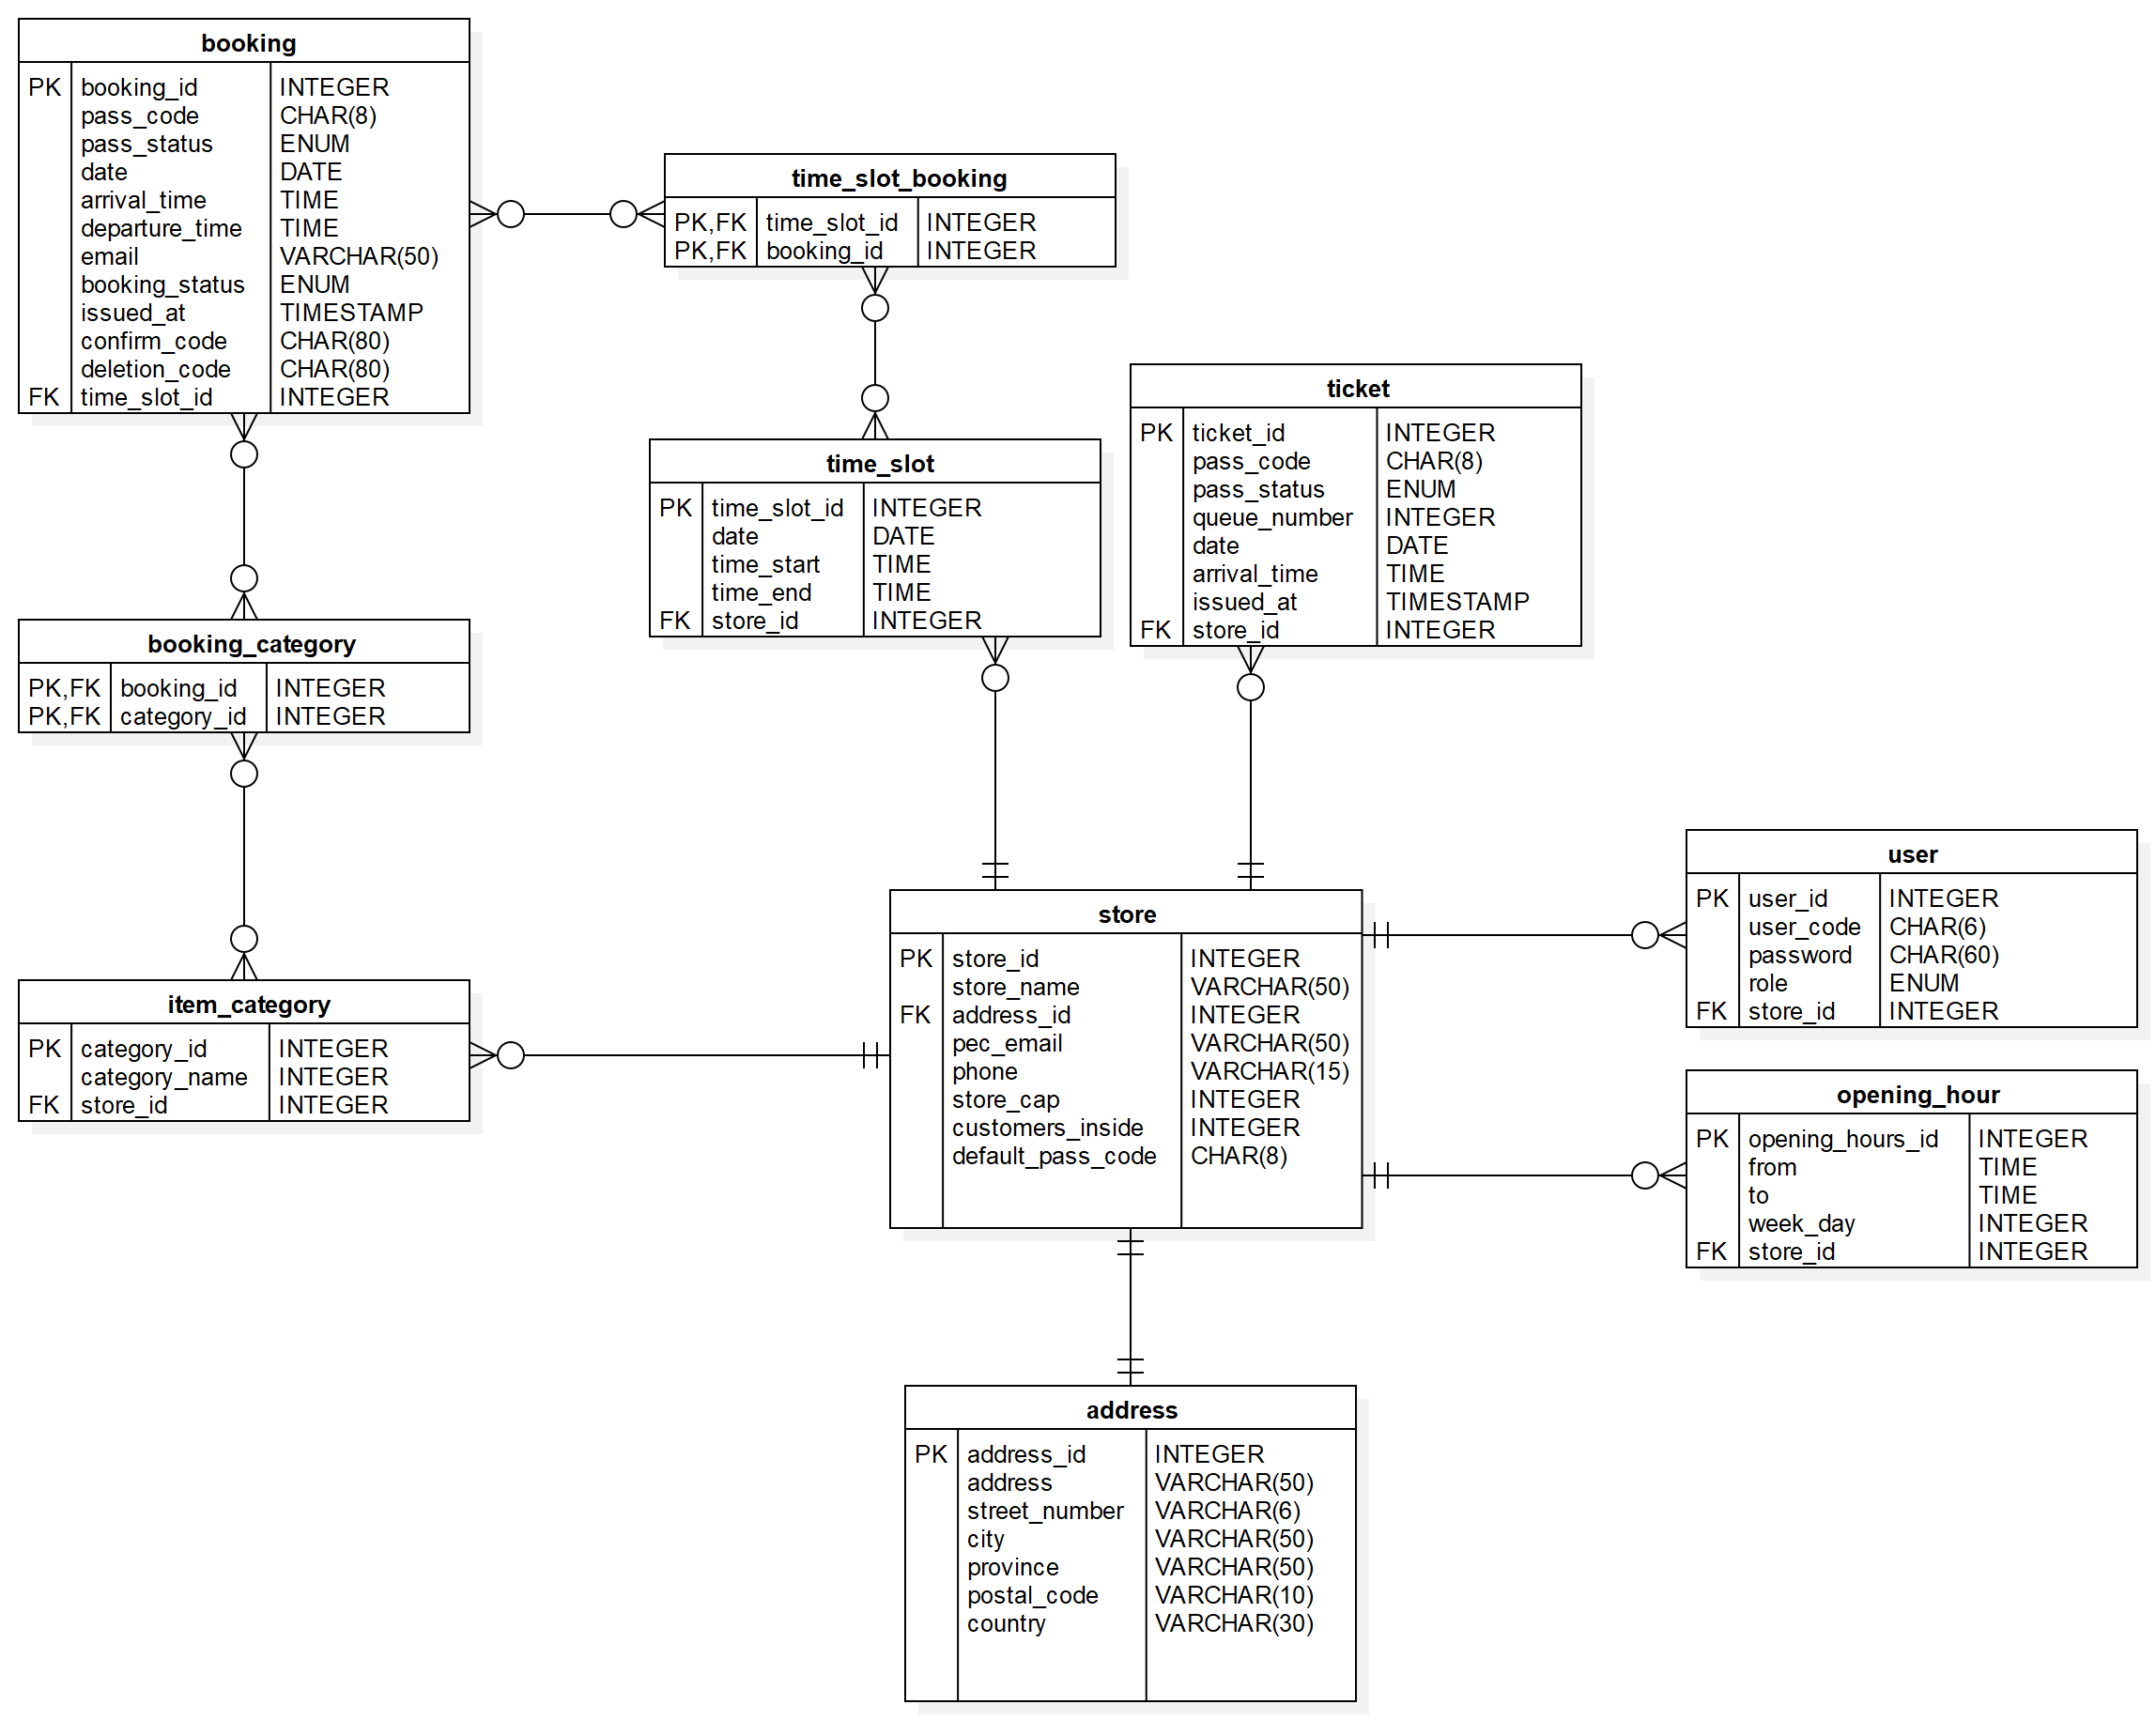
\includegraphics[width=\linewidth]{er_diagram}
	\caption{Database structure.}
	\label{fig:er_diagram}
\end{figure}

